\documentclass[a4paper,11pt]{article}
\author{ 杨旭鹏  \  PB17000234}
\date{2019年秋季}
\title{计算物理A 第五题}

\usepackage{ctex}
\usepackage{amsmath}
\usepackage{amsfonts}
\usepackage{graphicx}
\usepackage{lastpage}
\usepackage{hyperref}
\usepackage{listings}
\RequirePackage{xcolor}
\usepackage{appendix}
\usepackage{caption2}
\usepackage{subfigure}
\usepackage{float}
\makeatletter\def\@captype{table}\makeatother

\definecolor{dkgreen}{rgb}{0,0.6,0}
\definecolor{gray}{rgb}{0.5,0.5,0.5}
\definecolor{mauve}{rgb}{0.58,0,0.82}

\lstset{
  frame=tb,
  aboveskip=3mm,
  belowskip=3mm,
  showstringspaces=false,
  columns=flexible,
  framerule=1pt,
  rulecolor=\color{gray!35},
  backgroundcolor=\color{gray!5},
  basicstyle={\small\ttfamily},
  numbers=left,
  numberstyle=\tiny\color{gray},
  keywordstyle=\color{blue},
  commentstyle=\color{dkgreen},
  stringstyle=\color{mauve},
  breaklines=true,
  breakatwhitespace=true,
  tabsize=3,            
  }



\begin{document}
\maketitle

\section{题目描述}
对于球面上均匀分布的随机坐标点,给出它们在$(x, y)$平面上投影的几 率分布函数。并由此验证Marsaglia抽样方法 $x = 2u \sqrt{1-r ^{2} }, y = 2v \sqrt{1-r ^{2} } , z = 1 - 2r^{2}  $确为球面上均匀分布的随机抽样。




\section{算法}
\subsection{16807产生器}
16807产生器属于线性同余法产生器的特例。而线性同余法方法为:

\begin{equation}
\begin{aligned}
	I_{n+1} &= (aI_{n} + b) \ mod \ m \\
	x_{n} &= I_{n}/m
\end{aligned}
\label{linear}	
\end{equation}

其中整数$I_{i} \in [0,m-1]$,$a,b,m$为算法中的可调参数,其选取直接影响产生器的质量。选取参数:
\begin{equation}
\left\{
\begin{array}{l}
	a = 7^{5} = 16807 \\
	b = 0 \\
	m = 2^{31}-1 = 2147483647
\end{array}
\right.
\end{equation}

即为所谓的16807产生器。由于直接利用\ref{linear}编写程序时计算$(aI_{n} \ mod \ m )$时很容易造成数据溢出,故采取Schrage方法进行具体编程的实现:

\begin{equation}
	aI_{n} \ mod \ m = \left\{
	\begin{array}{l}
		a(I_{n}\ mod \ q) - r[I_{n}/q],\ \ \ \ \ \ \ \ if \geq 0 \\
		a(I_{n}\ mod \ q) - r[I_{n}/q] + m,\ \ otherwise	
			\end{array}
	\right.
\end{equation}

其中$m=aq+r$,即$q=m/a=127773$,$r=m \ mod \ a=2836$。即可利用此方法产生伪随机数序列。

\subsection{Fibonacci延迟产生器:Marsaglia 1号产生器}
其思想是用序列中的两个整数进行操作得到后续的整数,较线性同余法的优势在于它的周期非常长:
\begin{equation}
	I_{n}=I_{n-p} \otimes I_{n-q} \ mod \  m
\end{equation}
其中操作符$\otimes$可以是:“$+$”,“$-$”,“$\times$”,“XOR”。整数对$[p,q]$表示延迟,取值并非按Fibonacci数序列,而是根据统计验证后确认。

在此程序中,我们使用的是Fibonacci延迟产生器的一个特例——Marsaglia 1号 产生器:
\begin{equation}
	I_{n}=\left\{
	\begin{array}{l}
		I_{n-p} - I_{n-q},  \ \ \ \ \ \ \ if \geq 0 \\
		I_{n-p} - I_{n-q}+1, \ \ otherwise
	\end{array}
	\right.
\end{equation}
其中的$[p,q]$整数对的值选为$[97,33]$,因此其算法要求存储所有前面的97个随机数值。在本程序中,前97个随机数值由在Linux系统下访问“/dev/random”一次性来得到\footnote{对于Linux下的“/dev/random”文件在Linux manual page 上有如下解释:The random number generator gathers environmental noise from device
       drivers and other sources into an entropy pool.  The generator also
       keeps an estimate of the number of bits of noise in the entropy pool.
       From this entropy pool, random numbers are created.可以看出此种方法产生的随机数并非来自于算法,而来自于热噪声。},\footnote{便于结果的可重复性,方便调试程序}并存储为文件以便后期读取使用(此文件的原始数据见附录 \ref{971}和\ref{972})。



\subsection{Marsaglia抽样方法}
Marsaglia抽样方法本质上为一种舍选法,其思路大致为:
\begin{description} 
\item[1] 随机抽样一对均匀分布的随机数,$( u , v ) \in [ −1,1 ]$ ;
\item[2] 计算 $r^{2} = u^{2} + v^{2} $,如 果$ r^{2} > 1$ 则重新抽样直至$ r^{2} \leq 1$ ;
\item[3]则$x = 2u \sqrt{1 − r^{2} }, y = 2v \sqrt{1 − r^{2} }, z = 1 − 2r^{2} $即为三维球面上均匀分布的随机点。
\end{description}



\section{在$(x,y)$平面上投影的几率分布函数}

在本问题中,需要得到在球面上均匀分布的随机点,即在球面上任意位置,单位面积上点出现的概率为一定值。在某一球面上,半径$\rho$值是固定的,自变量仅为角度$\theta$和$\phi$。设概率密度函数为$p(\theta,\phi)$,则对于单位面积元上点出现的概率$d P$有:
\begin{equation}
	const = d P =p(\theta,\phi)d \theta d \phi dS^{2}
\end{equation}

当$d S^{2}= sin(\theta)d \theta d \phi $为定值时,我们有$d\theta \propto \frac{1}{sin(\theta)}$。则为了满足上式,我们有$p(\theta,\phi) \propto sin(\theta)$。设$p(\theta,\phi) = ksin(\theta)$,根据密度函数的归一性有

\begin{equation}
	1 = \int_{0}^{2\pi}\int_{0}^{\pi} k sin(\theta)d\theta d\phi 
\end{equation}
得到$k=\frac{1}{4\pi}$。即有$p(\theta,\phi)= p_{\theta}(\theta)p_{\phi}(\phi)=\frac{1}{4\pi}sin(\theta)$。

为了得到投影到$(x,y)$平面上的几率,我们设关于$(x,y)$的概率密度函数为$g(x,y)$,则有:\footnote{这里不妨假设球面半径为1,方便计算}
\begin{equation}
\left\{
\begin{array}{l}
	g(x,y)dxdy = p(\theta,\phi)d\theta d\phi = \frac{sin(\theta)}{4\pi}d\theta d\phi \\
	x=sin(\theta)cos(\phi) \\
	y=sin(\theta)sin(\phi)
\end{array}	
\right.
\end{equation}

我们利用jacobi行列式将上式进行换元操作有:
\begin{equation}
\begin{aligned}
	\frac{sin(\theta)}{4\pi} d\theta d\phi &= g(x,y)\left| \frac{\partial(x,y)}{\partial(\theta,\phi)} \right| d\theta d\phi \\
	&= g(x,y) \left| cos(\theta)sin(\theta) \right| d\theta d\phi
\end{aligned}
\end{equation}
继续化简上式得到:
\begin{equation}
	g(x,y) = \frac{1}{4\pi \sqrt{1-x^{2}-y^{2}}}
\end{equation}


\section{验证Marsaglia抽样方法确为球面上均匀分布的随机抽样}

我们有:
\begin{equation}
	h(u,v)dudv = g(x,y)dxdy = g(x,y)\left| \frac{\partial(x,y)}{\partial(u,v)} \right| du dv
\end{equation}

带入$x,y$与$u,v$的关系式:
\begin{equation}
\left\{
\begin{array}{l}
	x = 2u \sqrt{1 − r^{2} }\\
	y = 2v \sqrt{1 − r^{2} } \\
	r^{2} = u^{2}+v^{2}
\end{array}
\right.
\end{equation}
得到:
\begin{equation}
	g(x,y) = \frac{h(u,v)}{|4 - 8 u^{2} - 8 v^{2}|} = \frac{1}{4\pi\sqrt{1-x^{2}-y^{2}}}
\end{equation}
其中$h(u,v) = \frac{1}{\pi}$。可知其表达式与球面均匀分布点在$(x,y)$平面上的投影的概率密度函数相等。

我们又有:
\begin{equation}
	h(u,v)dudv = g(x,z)dxdz = g(x,z)\left| \frac{\partial(x,z)}{\partial(u,v)} \right| du dv
\end{equation}
带入关系式:
\begin{equation}
\left\{
\begin{array}{l}
	x = 2u \sqrt{1 − r^{2} }\\
	z = 1-2r^{2} \\
	r^{2} = u^{2}+v^{2}
\end{array}
\right.
\end{equation}
有:
\begin{equation}
	g(x,z) = \frac{h(u,v)}{|8v\sqrt{1-u^{2}-v^{2}}|} = \frac{1}{4\pi\sqrt{1-x^{2}-z^{2}}}
\end{equation}
其中$h(u,v) = \frac{1}{\pi}$。可知其表达式与球面均匀分布点在$(x,z)$平面上的投影的概率密度函数相等(由于点在球面上均匀分布,则在$(x,z)$平面上的投影的概率密度函数与在$(x,y)$平面上的投影的概率密度函数相等)。


根据Marsaglia抽样方法中$x,y$的对称性,球面的对称性,得到Marsaglia抽样方法在$(x,y)$,$(x,z)$,$(y,z)$平面上的投影的概率密度函数与球面上均匀分布的点在$(x,y)$,$(x,z)$,$(y,z)$平面上的投影的概率密度函数相等。则证明了利用Marsaglia抽样方法得到的随机点确为球面上均匀分布的随机点。




\section{程序思路}
对于Marsaglia 抽样方法,其随机数对$(u,v)$由16807产生器产生。对于16807产生器,其程序需要一个种子,在本程序中需要产生两组互不相关的随机数,则需要2个“互不相关”的初始种子值。这两个种子值通过一次性读取“/dev/random”文件得到,分别为34028207和1677078722\footnote{在这里我们这么做是为了结果的可重复性}。

产生随机种子后,各自利用递推公式:
\begin{equation}
	I_{n+1} = aI_{n}  \ mod \ m = \left\{
	\begin{array}{l}
	a(I_{n}\ mod \ q) - r[I_{n}/q],\ \ \ \ \ \ \ \ if \geq 0 \\
		a(I_{n}\ mod \ q) - r[I_{n}/q] + m,\ \ otherwise	 \\
		a= 7^{5} =16807 \\
		q=m/a=127773\\
		r=m \ mod \ a=2836
	\end{array} 
	\right.
\end{equation}

计算随机数列。

对于Marsaglia 1号 产生器,所需要97个初始随机数,得到方式在上文已经提及。

之后将产生的随机数组对$(u,v)$使用上文提到的舍取方法得到我们需要的随机点的$(x,y,z)$坐标值,存入文件,利用python可视化脚本画图。
详情请见代码。

\section{程序使用方法}
在运行程序后,会看到请求输入所需总随机点数的提示,按照提示在后面输入所需要的总随机点数,摁回车继续。然后按照程序提示,输入Marsaglia 1号产生器所需延迟整数值$[p,q]$(最大值不可超过97,Marsaglia 1号 产生器简易使用默认延迟整数值为$[97,33]$,建议按此输入),按回车继续程序。然后经过计算给出16807方法和Marsaglia方法产生的随机坐标$(\theta,\phi)$分别存为两个文件。程序输出完这些后会自动退出。
\begin{figure}[!htbp]        
\center{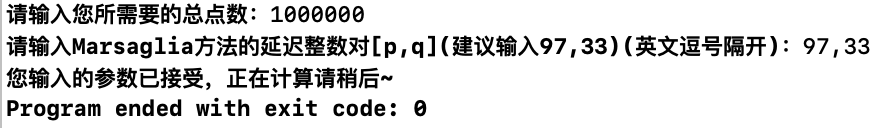
\includegraphics[width=10cm]  {example.png}}        
\caption{\label{1} 一个典型程序的运行过程示例}      
\end{figure}

\newpage
\section{程序结果与讨论}
当输入一些不同的点数时,得到如下结果:

\begin{figure}[!htbp]   
\centering     
\subfigure[默认视图]{
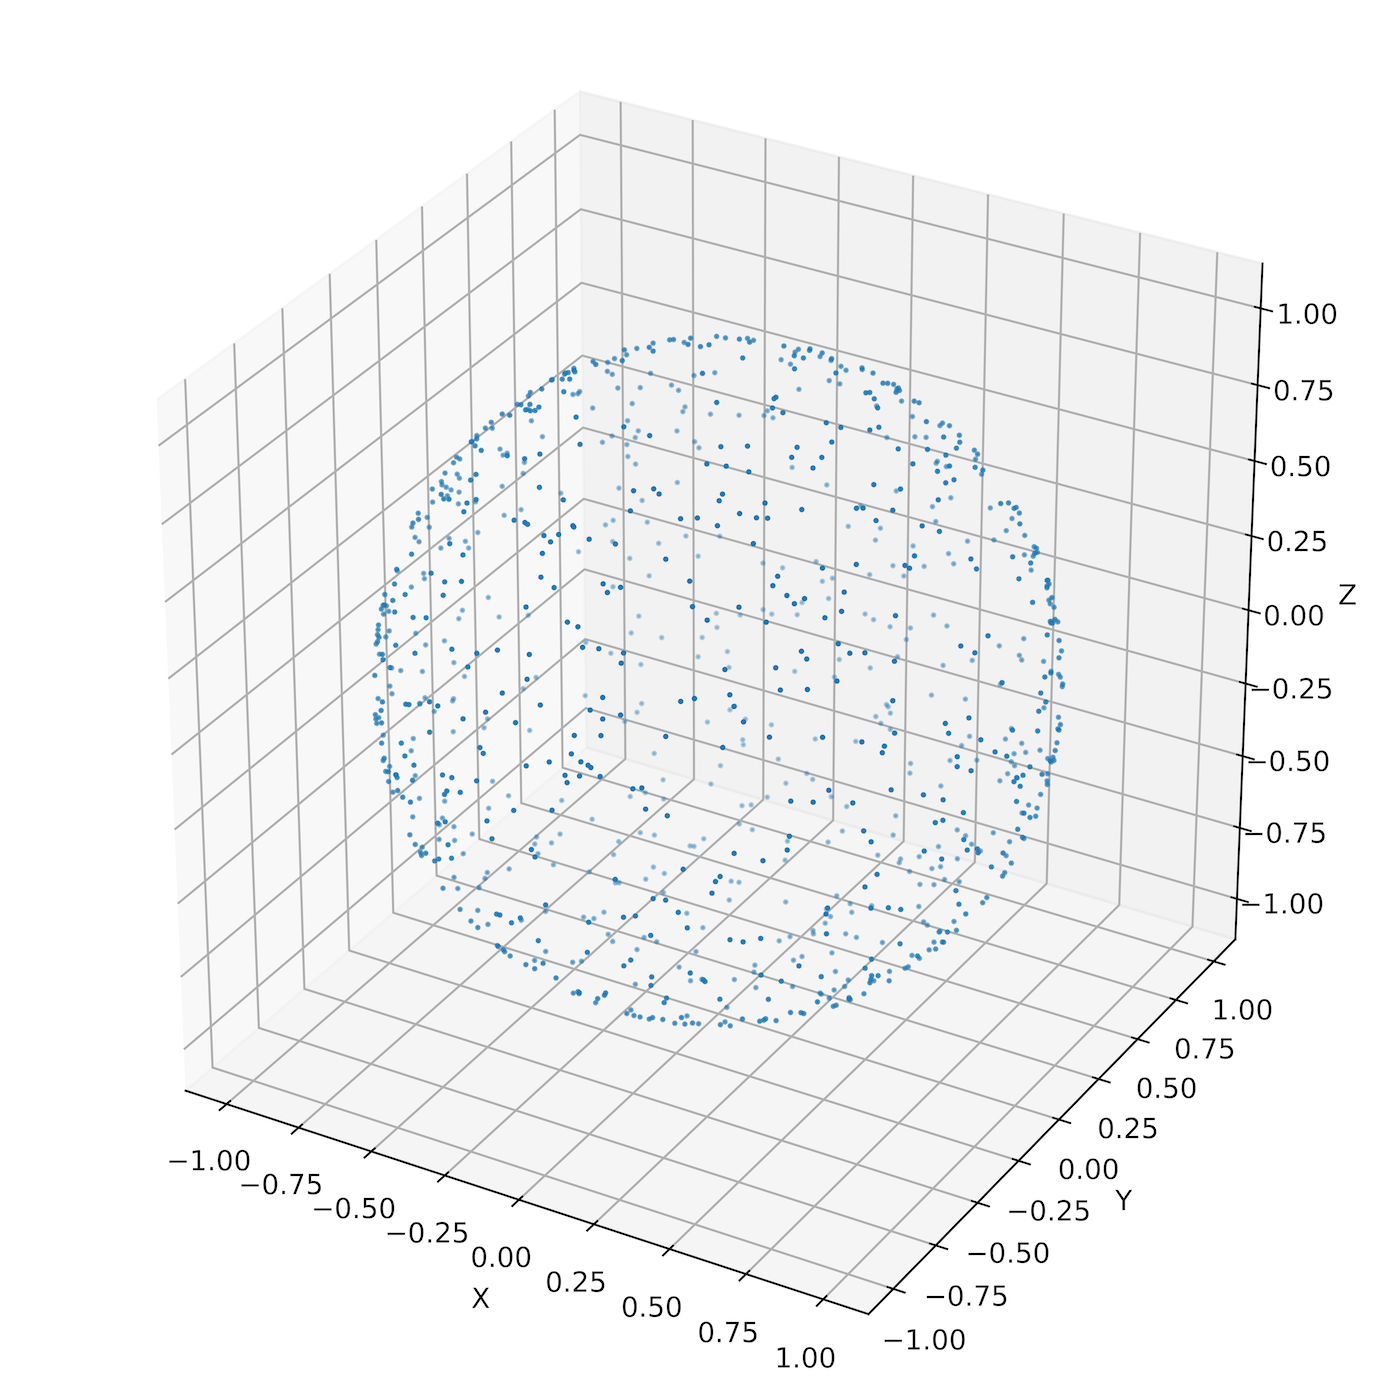
\includegraphics[width=6cm] {103.png}
}
\subfigure[z方向视图]{
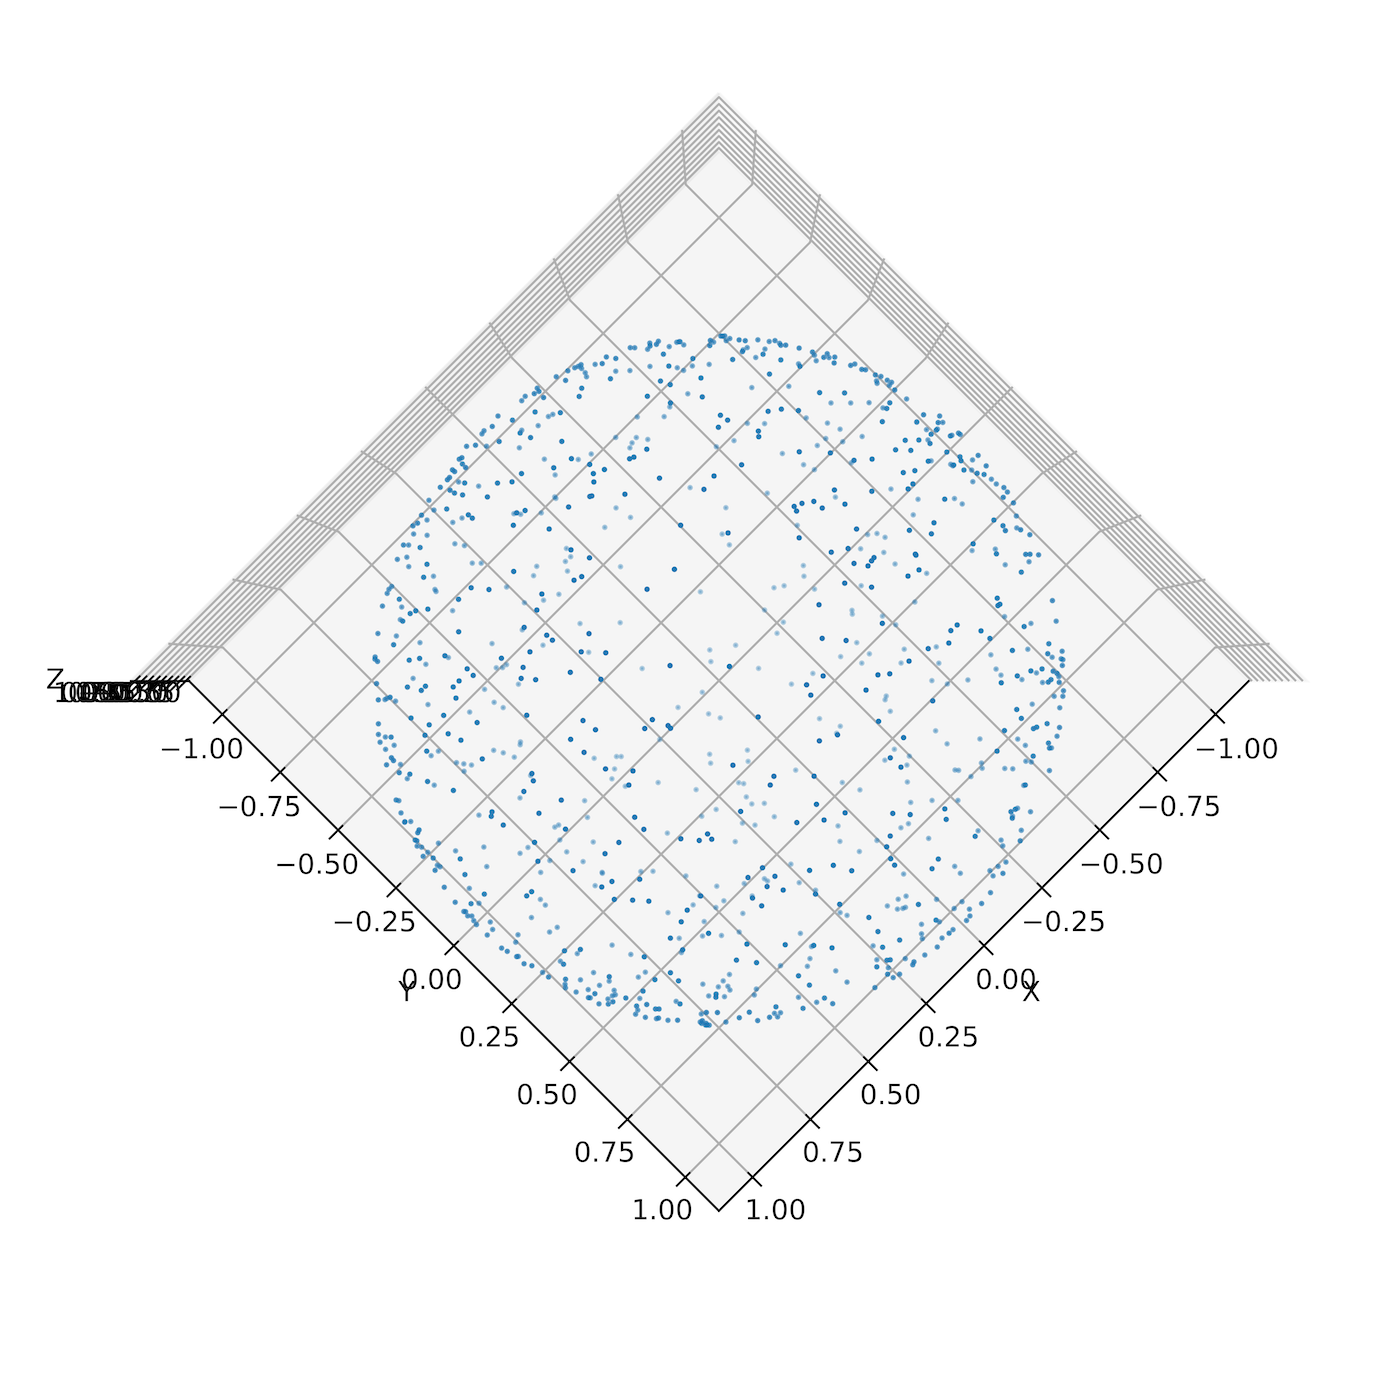
\includegraphics[width=6cm] {103-v.png}
}      
\caption{球面上均匀分布的1000随机点}      
\end{figure}

\begin{figure}[!htbp]   
\centering     
\subfigure[默认视图]{
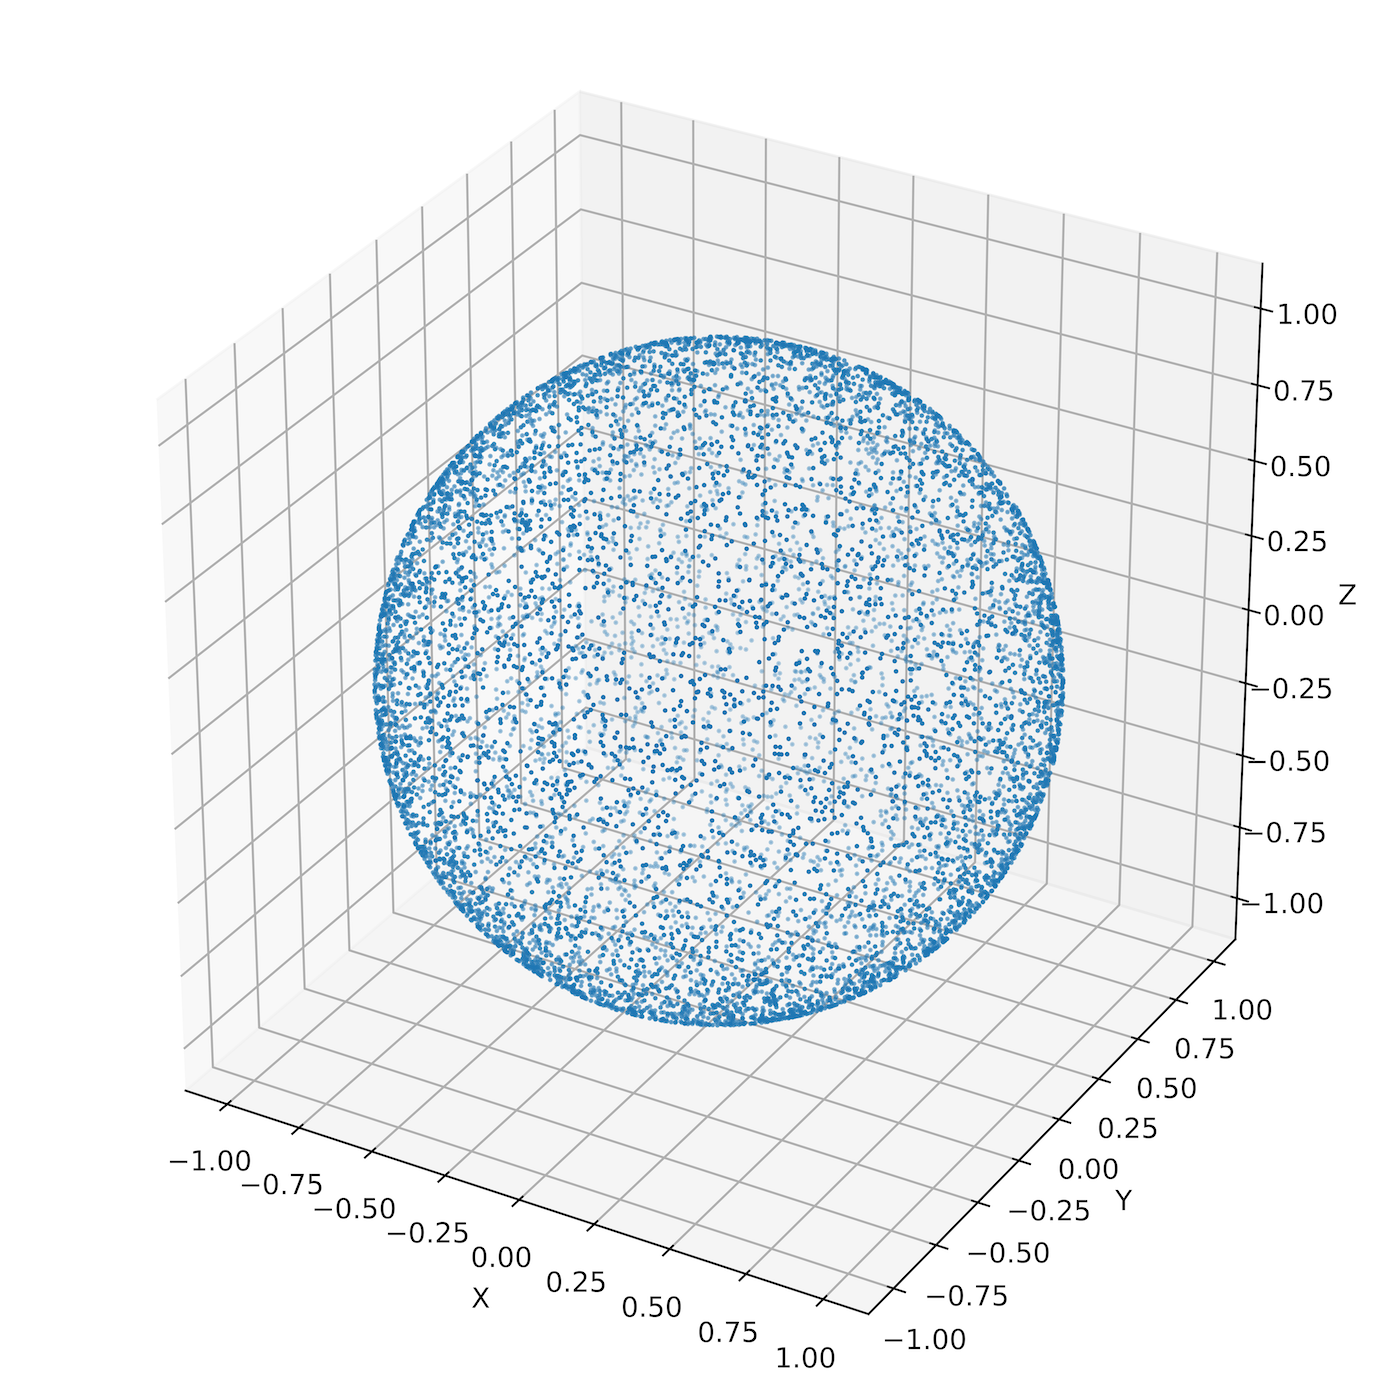
\includegraphics[width=6cm] {104.png}
}
\subfigure[z方向视图]{
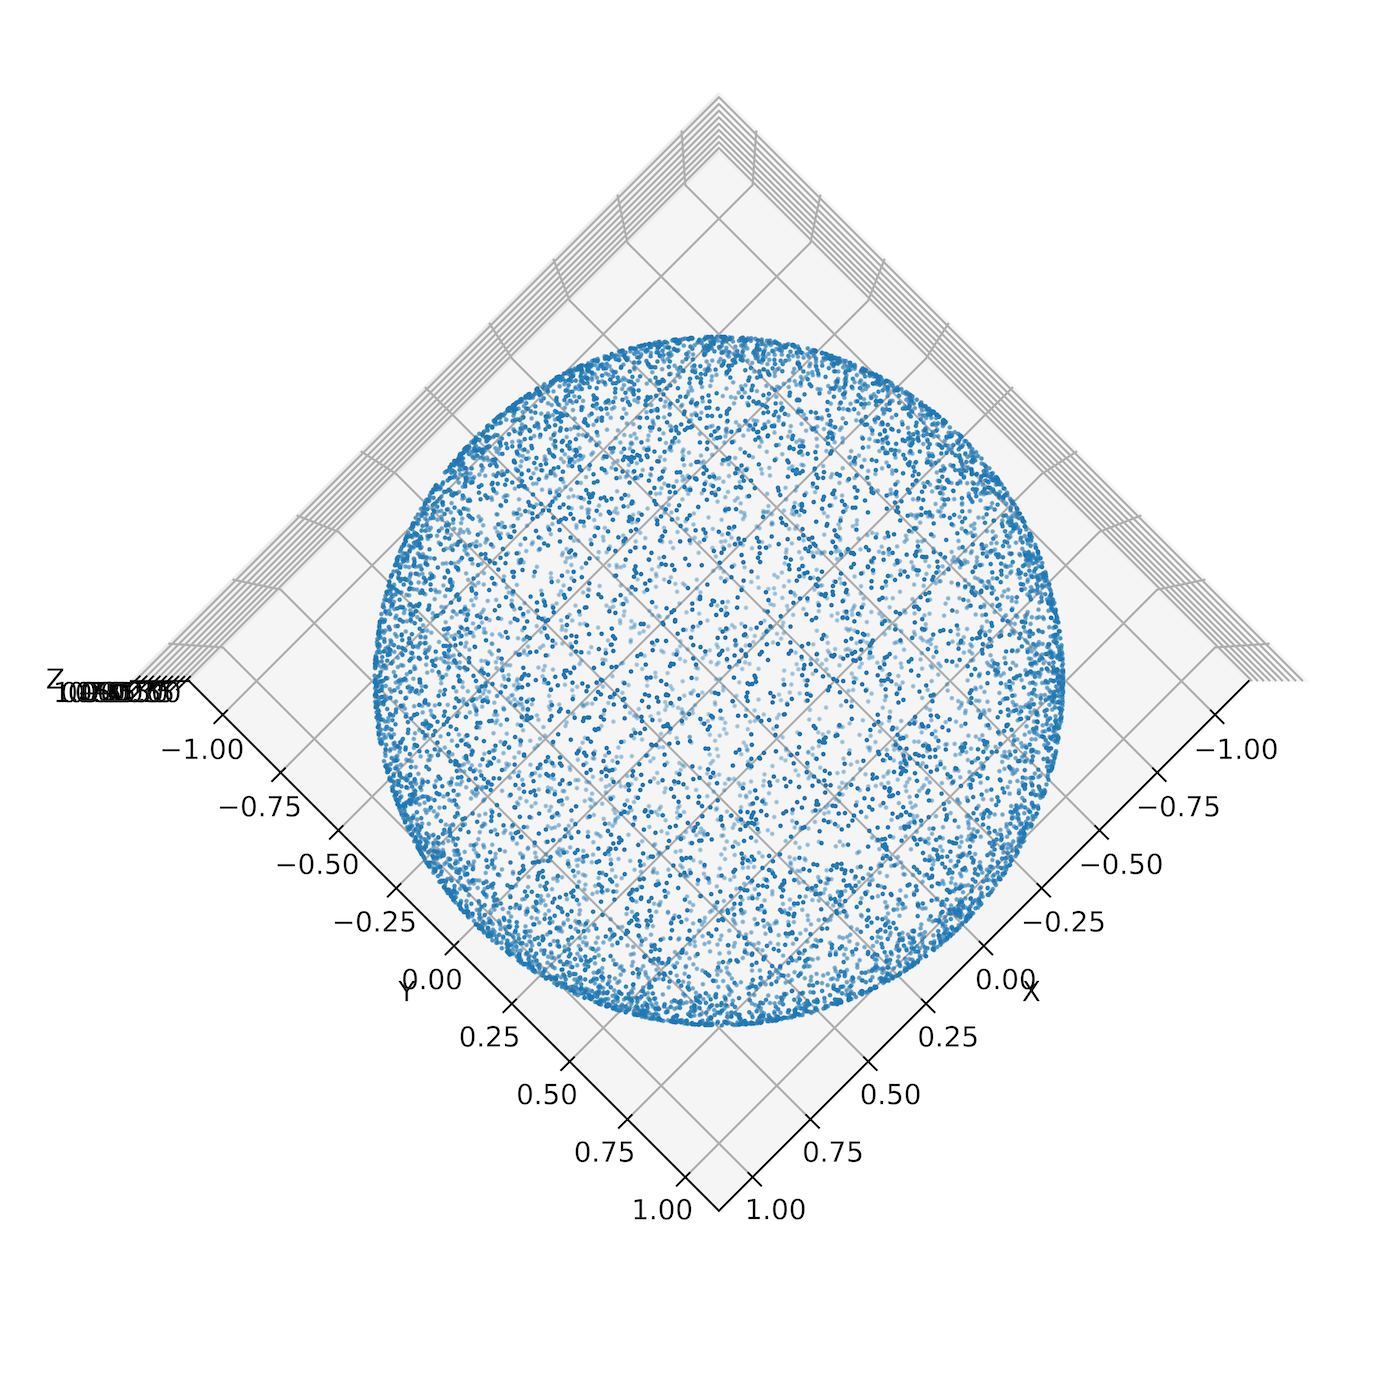
\includegraphics[width=6cm] {104-v.png}
}      
\caption{球面上均匀分布的$10^{4}$随机点}      
\end{figure}

\begin{figure}[!htbp]   
\centering     
\subfigure[默认视图]{
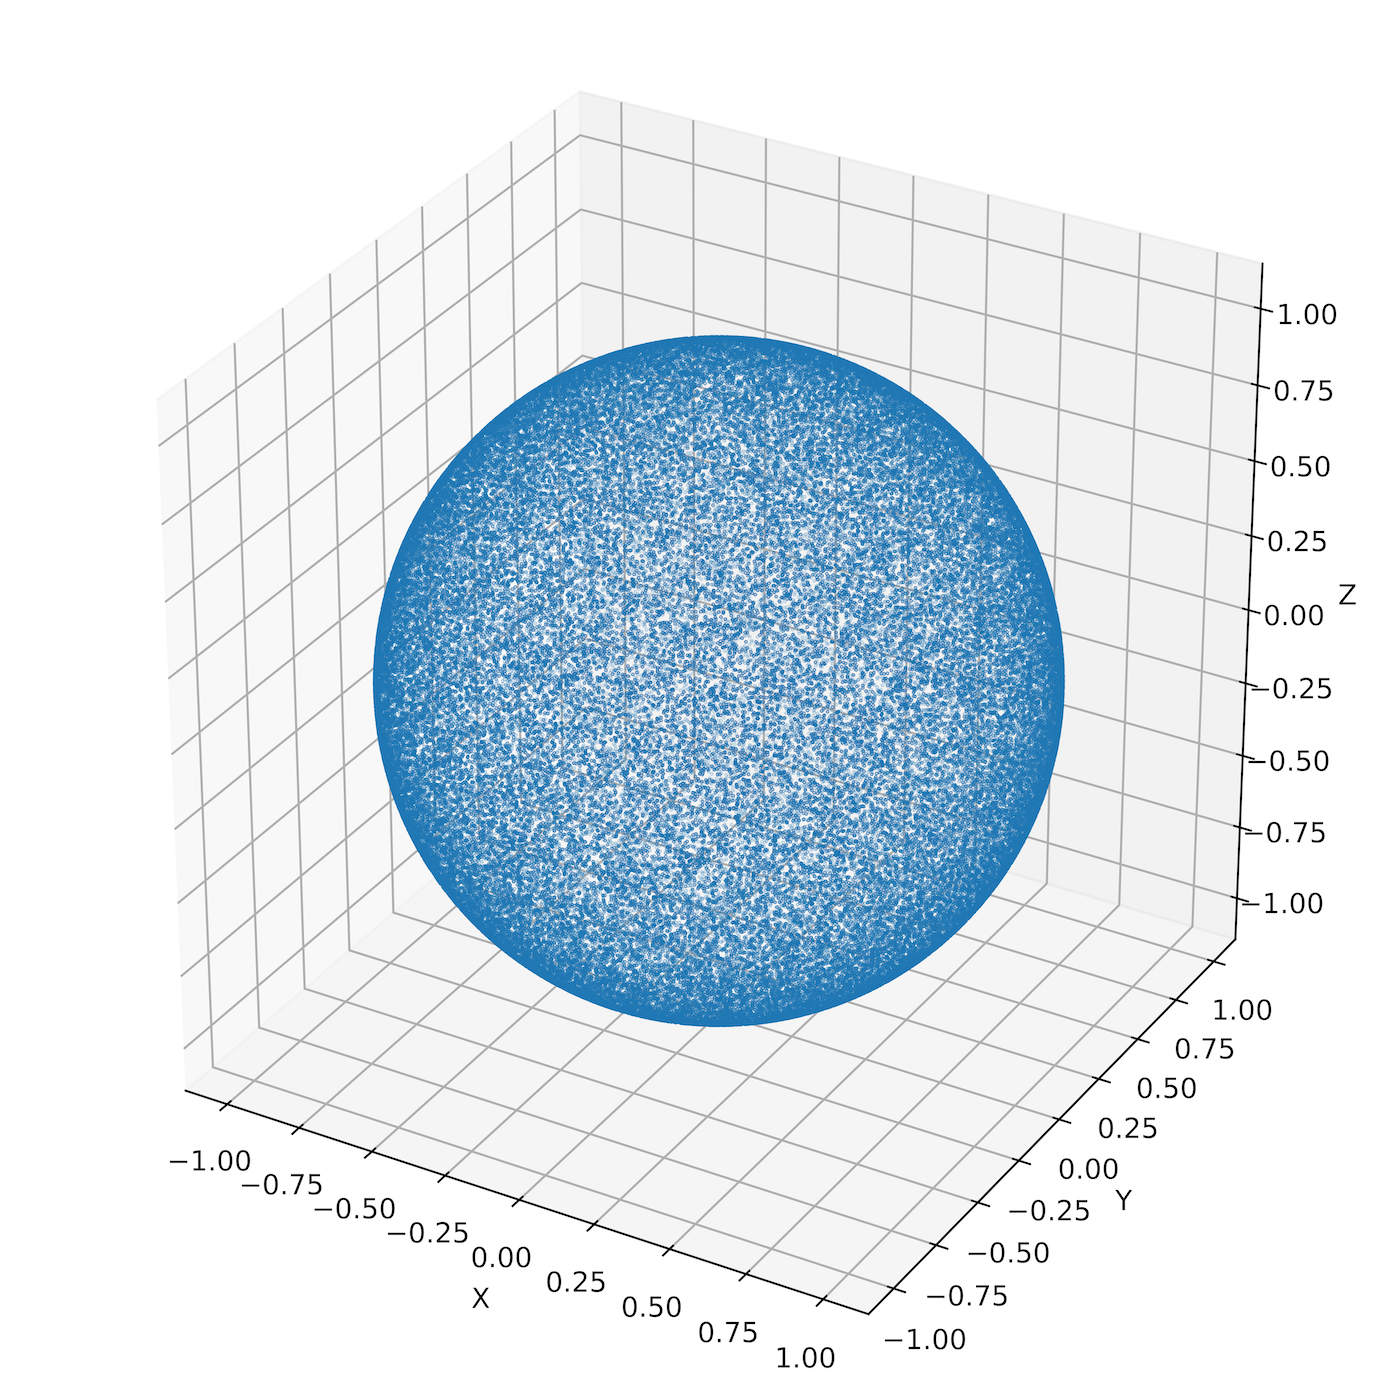
\includegraphics[width=6cm] {105.png}
}
\subfigure[z方向视图]{
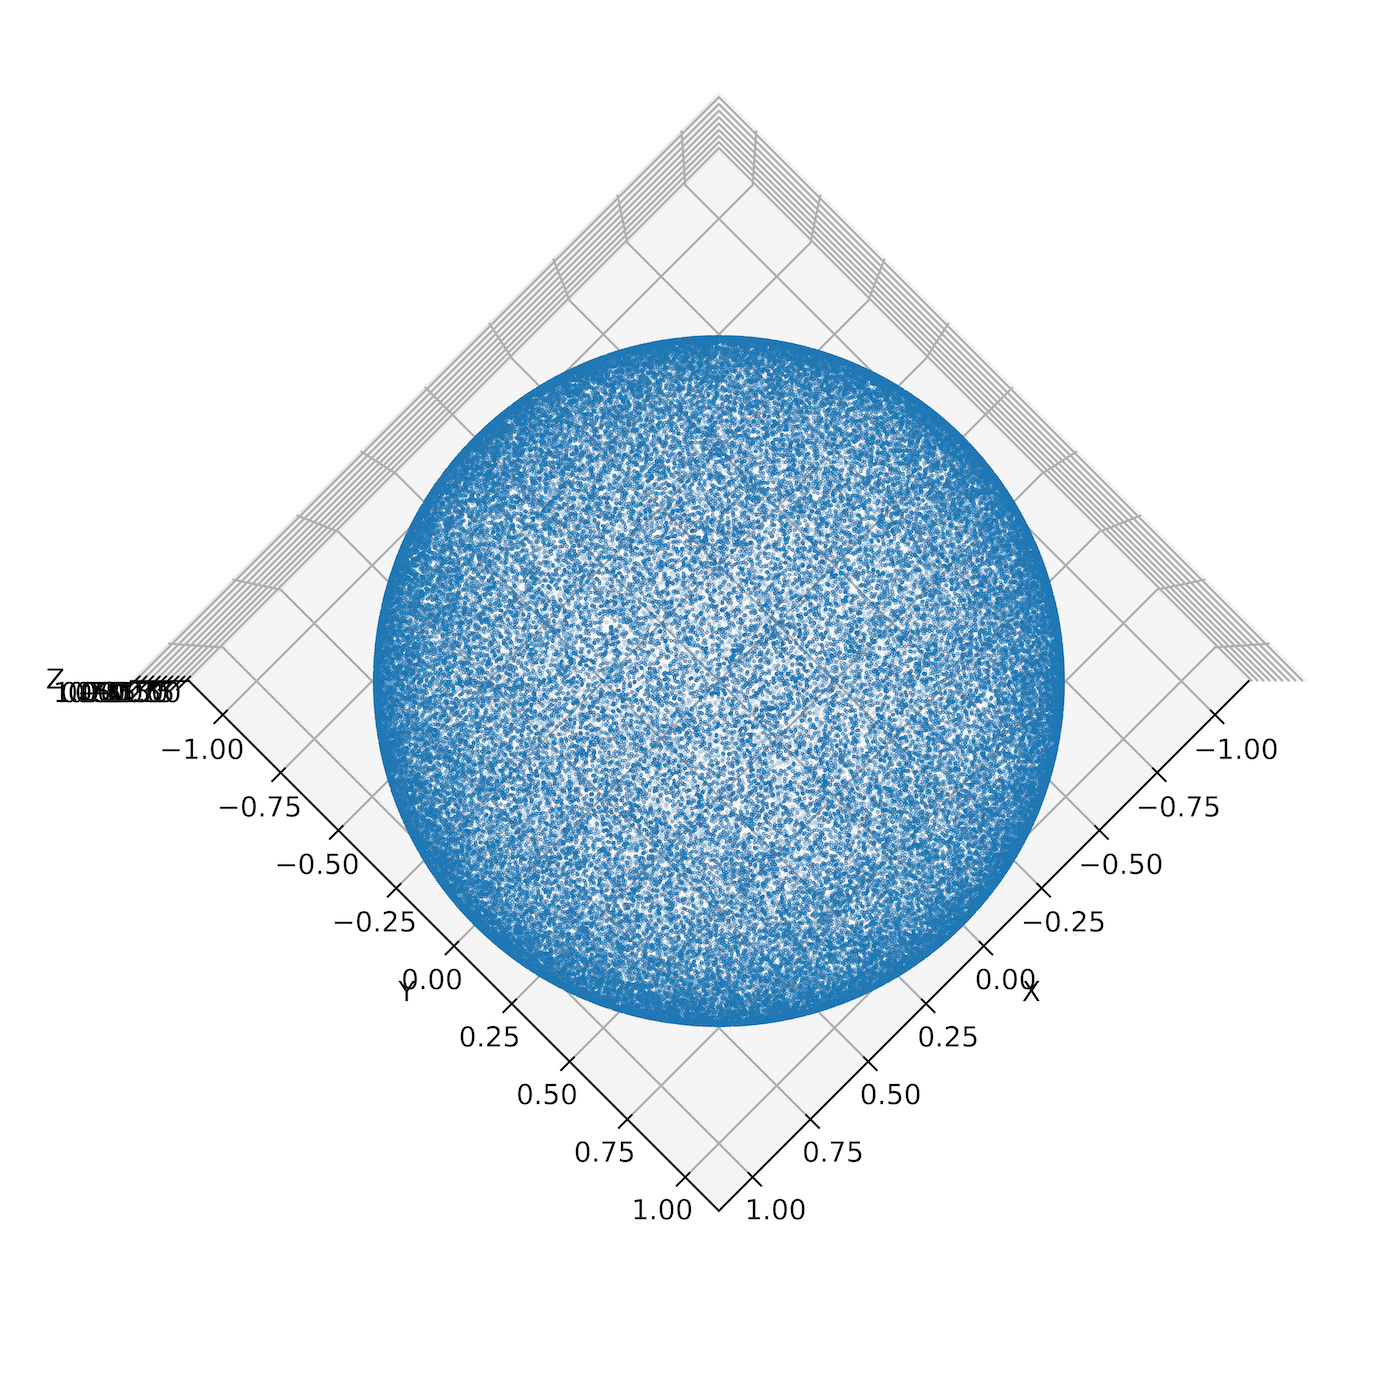
\includegraphics[width=6cm] {105-v.png}
}      
\caption{球面上均匀分布的$10^{5}$随机点}      
\end{figure}

\begin{figure}[!htbp]   
\centering     
\subfigure[默认视图]{
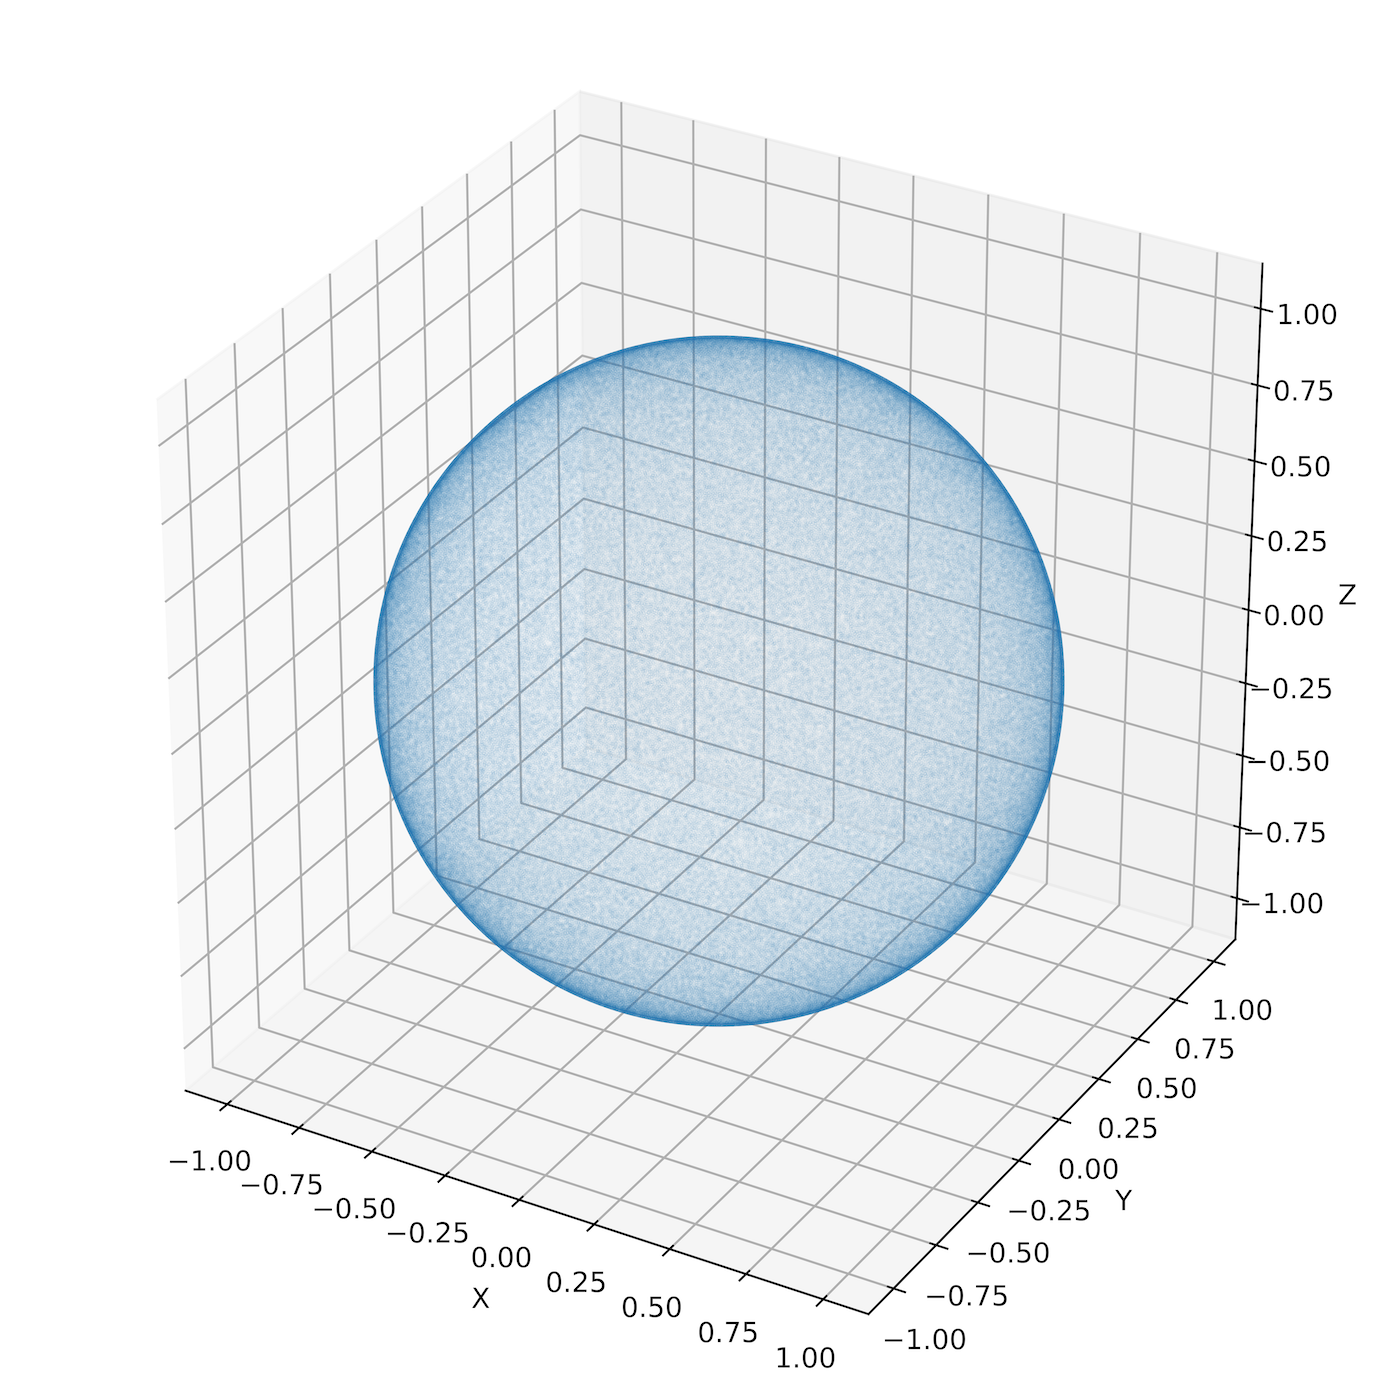
\includegraphics[width=6cm] {106.png}
}
\subfigure[z方向视图]{
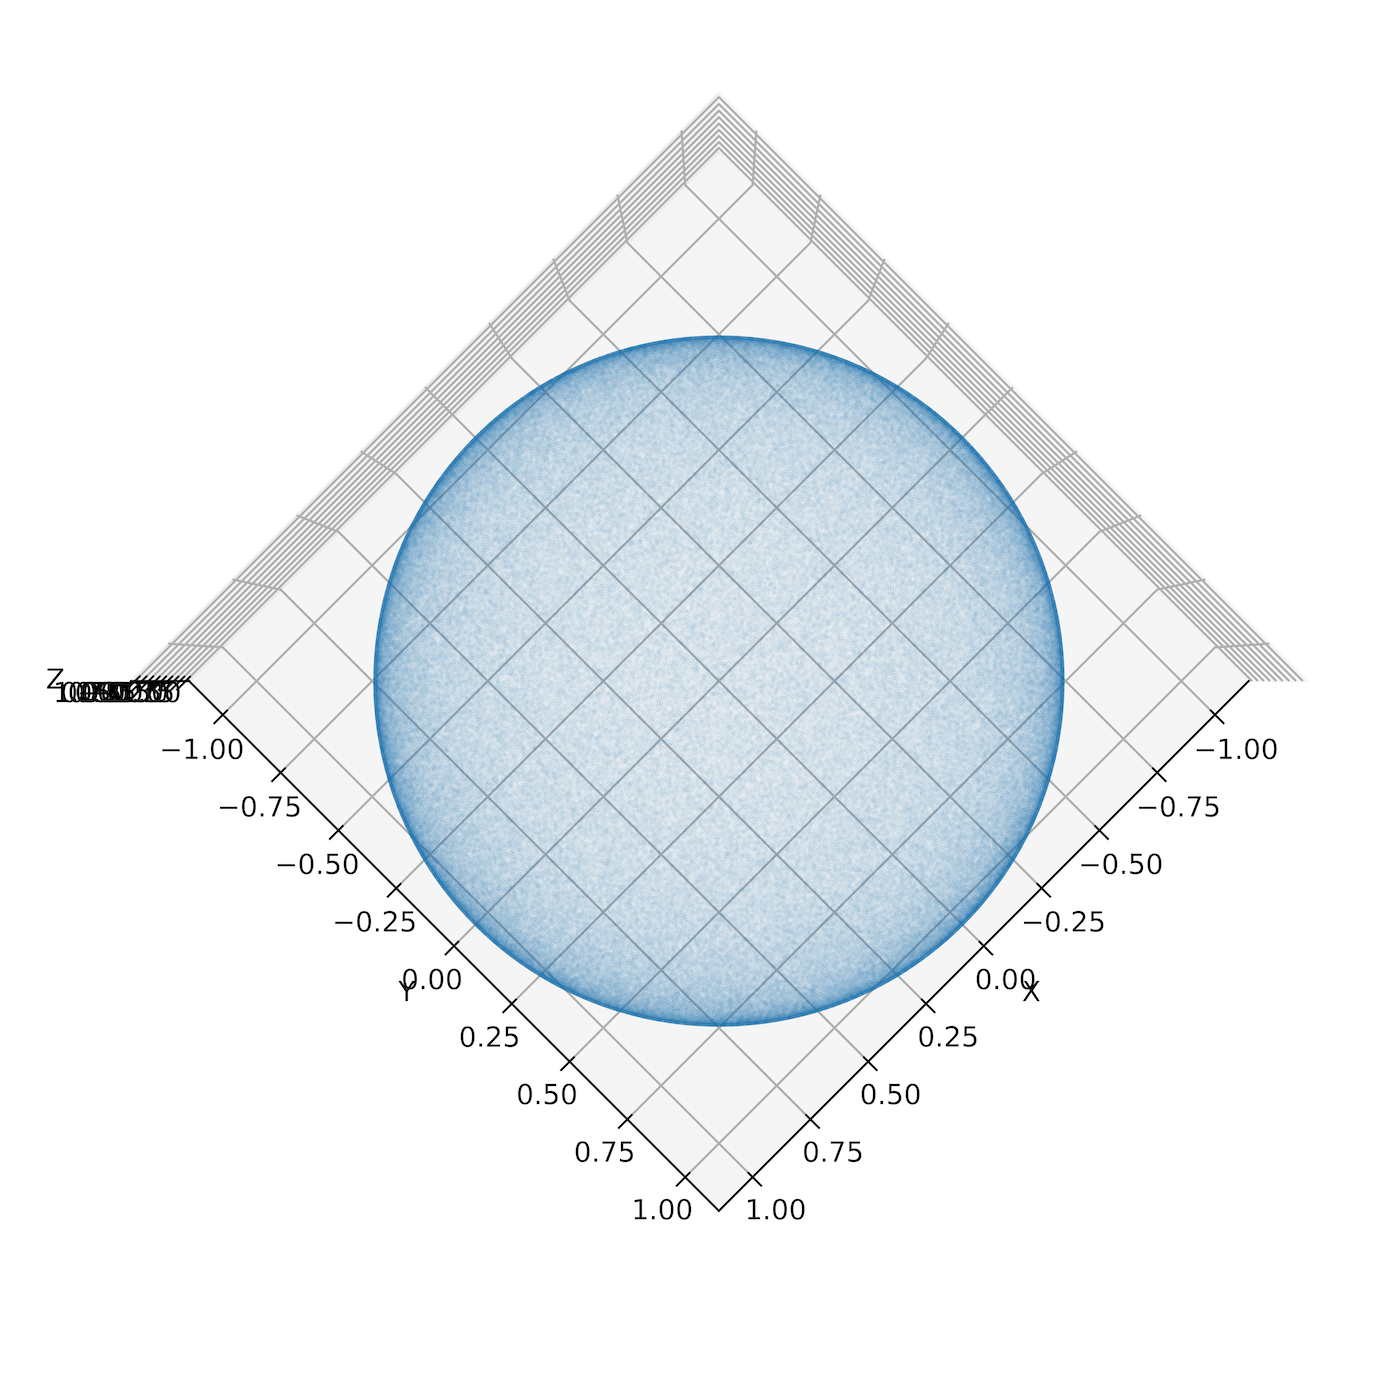
\includegraphics[width=6cm] {106-v.png}
}      
\caption{球面上均匀分布的$10^{6}$随机点}      
\end{figure}

\newpage
 由上述结果可以看出当$N\leq 10^{6}$时,利用16807和Marsaglia抽取相结合的方法产生的随机点在球面上的分布还算均匀,几乎看不出什么条带结构和规则网格结构等有明显规律性的结构。我们换取Marsaglia 1 号产生器和Marsaglia抽取法相结合的方式进行试验,得到如下结果:

\begin{figure}[!htbp]   
\centering     
\subfigure[默认视图]{
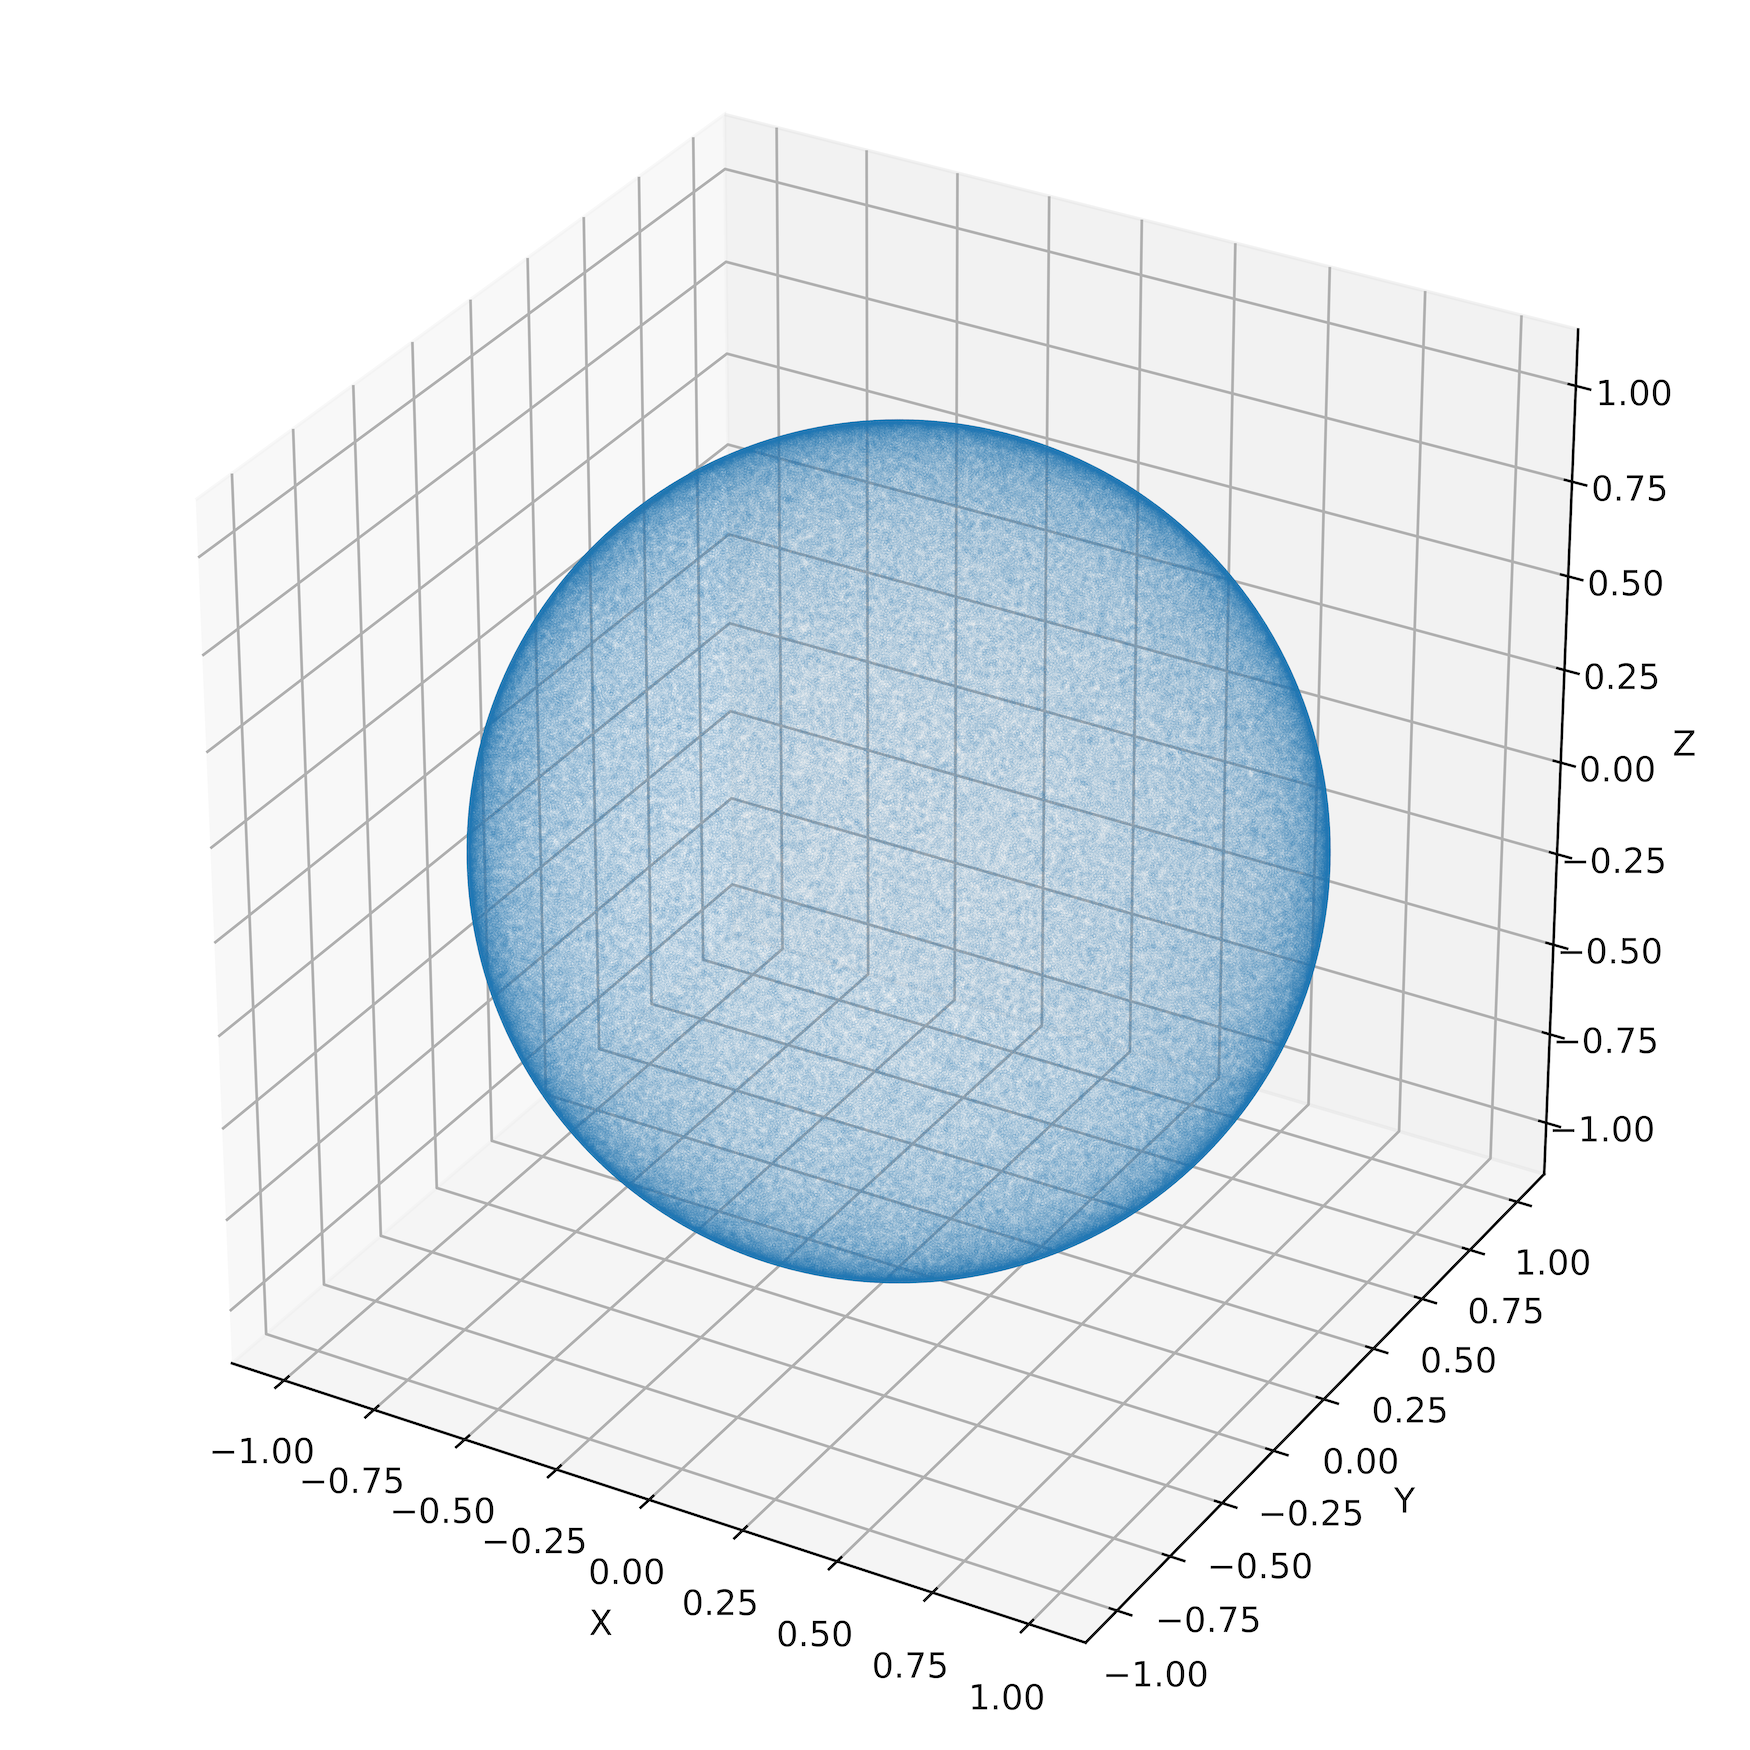
\includegraphics[width=7cm] {106-fibo.png}
}
\subfigure[z方向视图]{
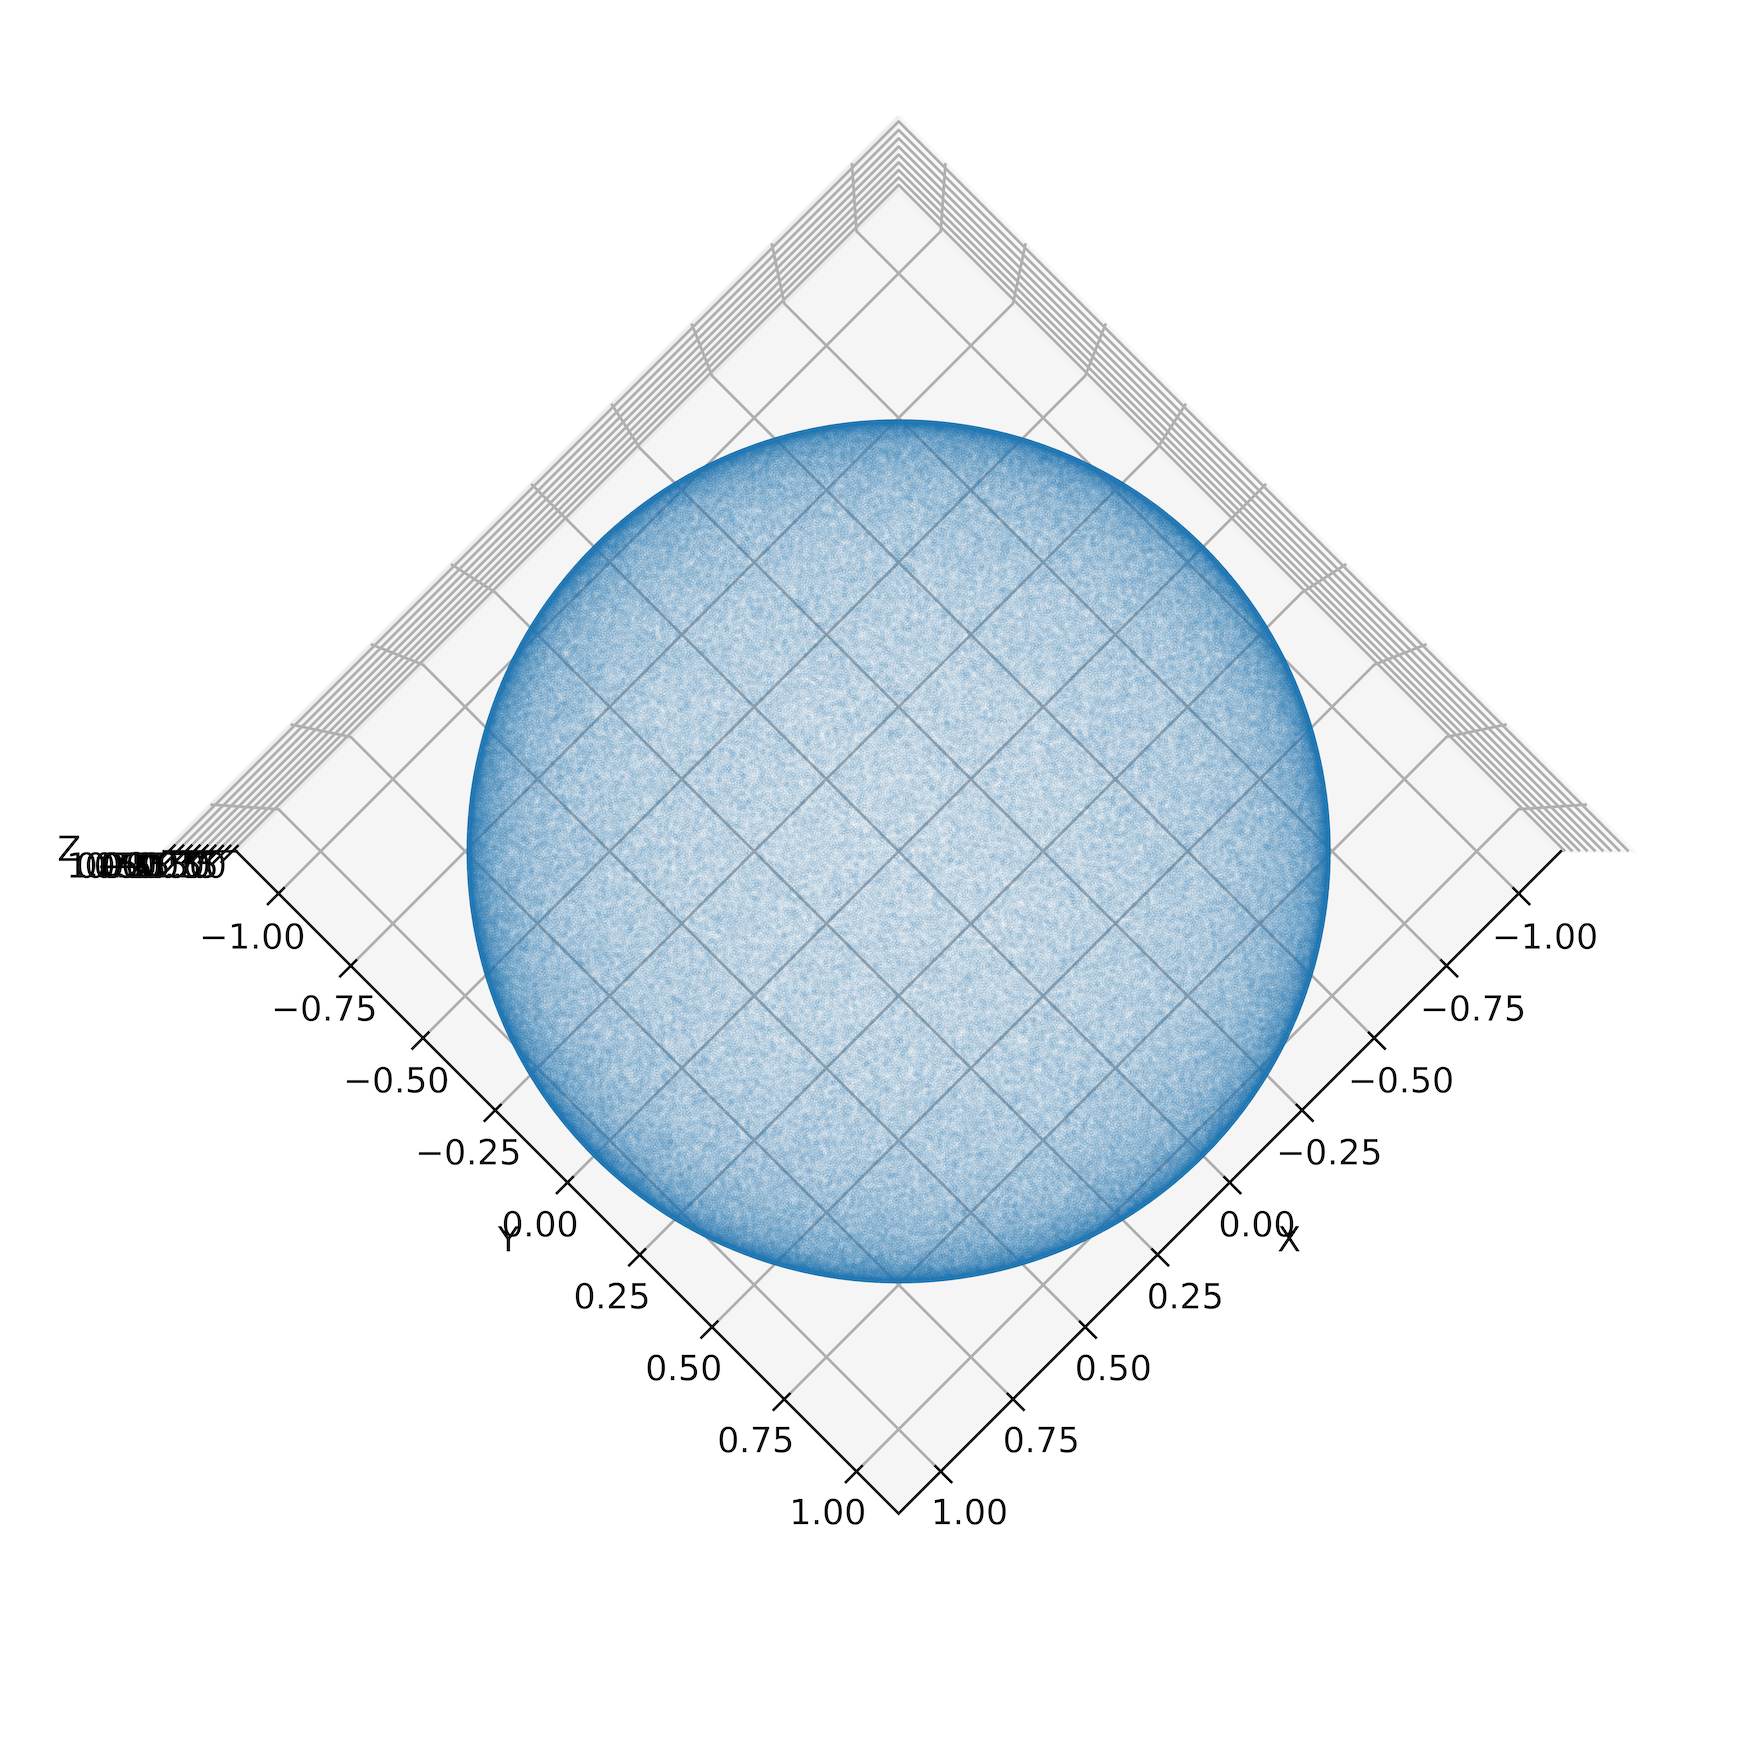
\includegraphics[width=7cm] {106-fibo-v.png}
}      
\caption{Marsaglia 1 号产生器产生的球面上均匀分布的$10^{6}$随机点}      
\end{figure}

\clearpage
可以看出利用marsaglia 1号产生器与Marsaglia抽取法相结合的方式产生的球面上均匀分布的随机点在$N=10^{6}$时看不出什么有规律性的结构,仍可认为是比较均匀的。

将$(x,y)$平面上的区域$[-1,1]\times [-1,1]$划分为$50\times 50$个小格,统计数值抽样后,每个小格内出现点的概率得到如下结果\footnote{可视化结果通过python脚本得到,由于点数相对于剖分区域还是比较少,故在靠近边缘处出现“毛刺”}:

\begin{figure}[!htbp]   
\centering     
\subfigure[默认视图]{
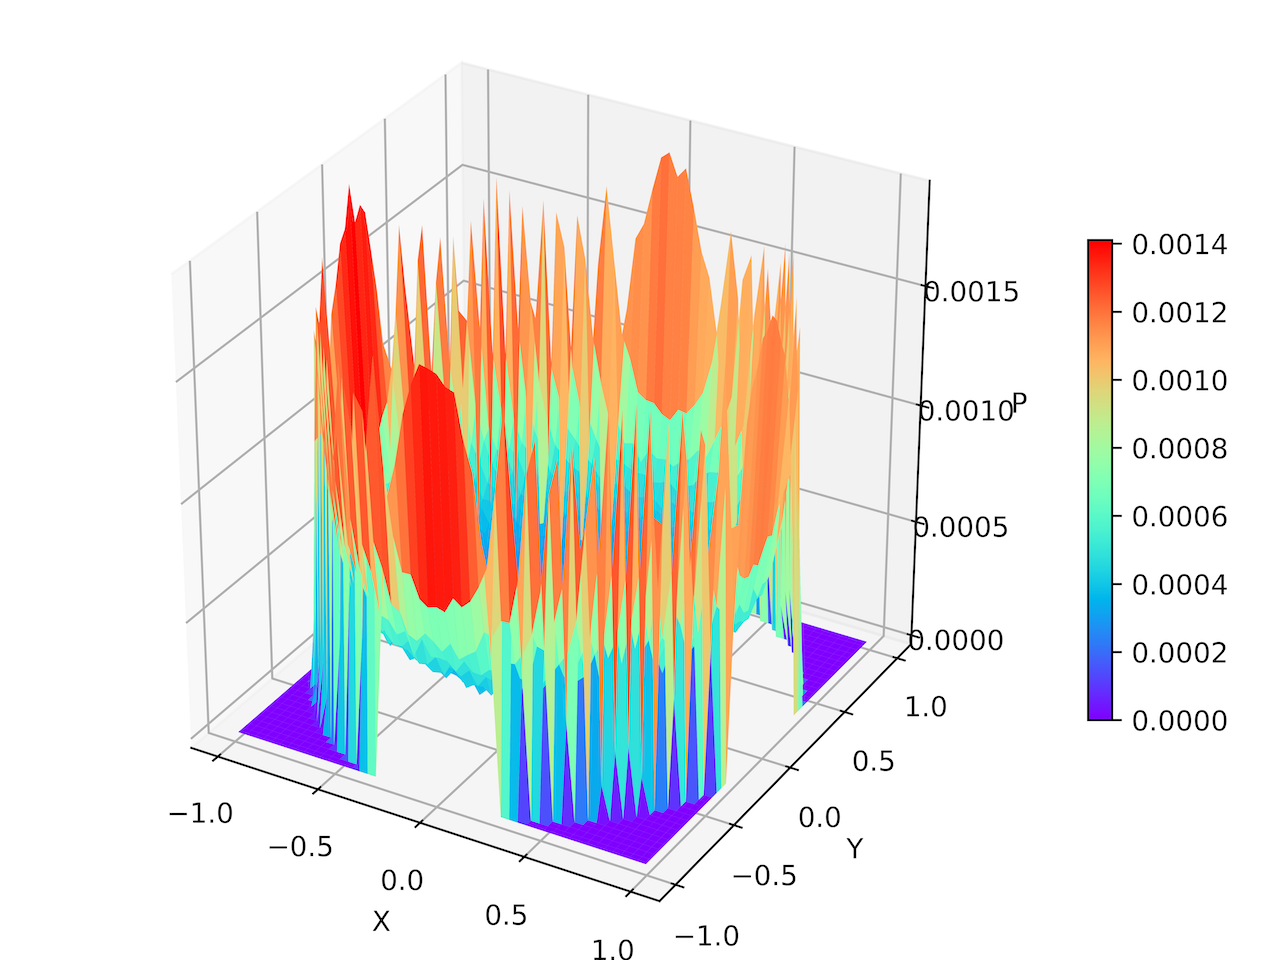
\includegraphics[width=5cm] {p106.png}
}
\subfigure[z方向视图]{
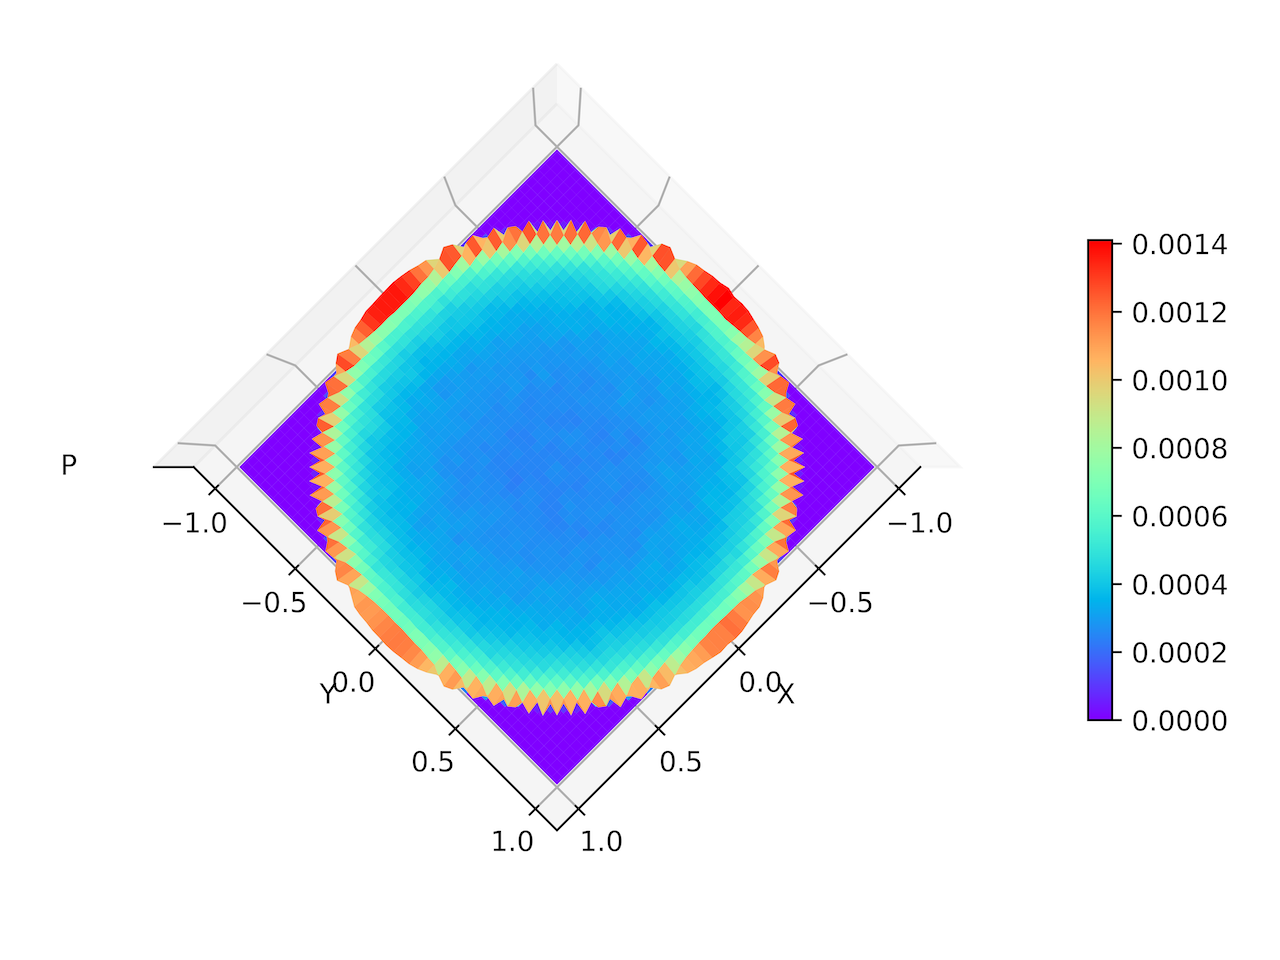
\includegraphics[width=5cm] {p106-v.png}
}      
\caption{16807 号产生器产生的球面上均匀分布的$10^{6}$随机点在$(x,y)$平面上的投影概率统计}      
\end{figure}

\begin{figure}[!htbp]   
\centering     
\subfigure[默认视图]{
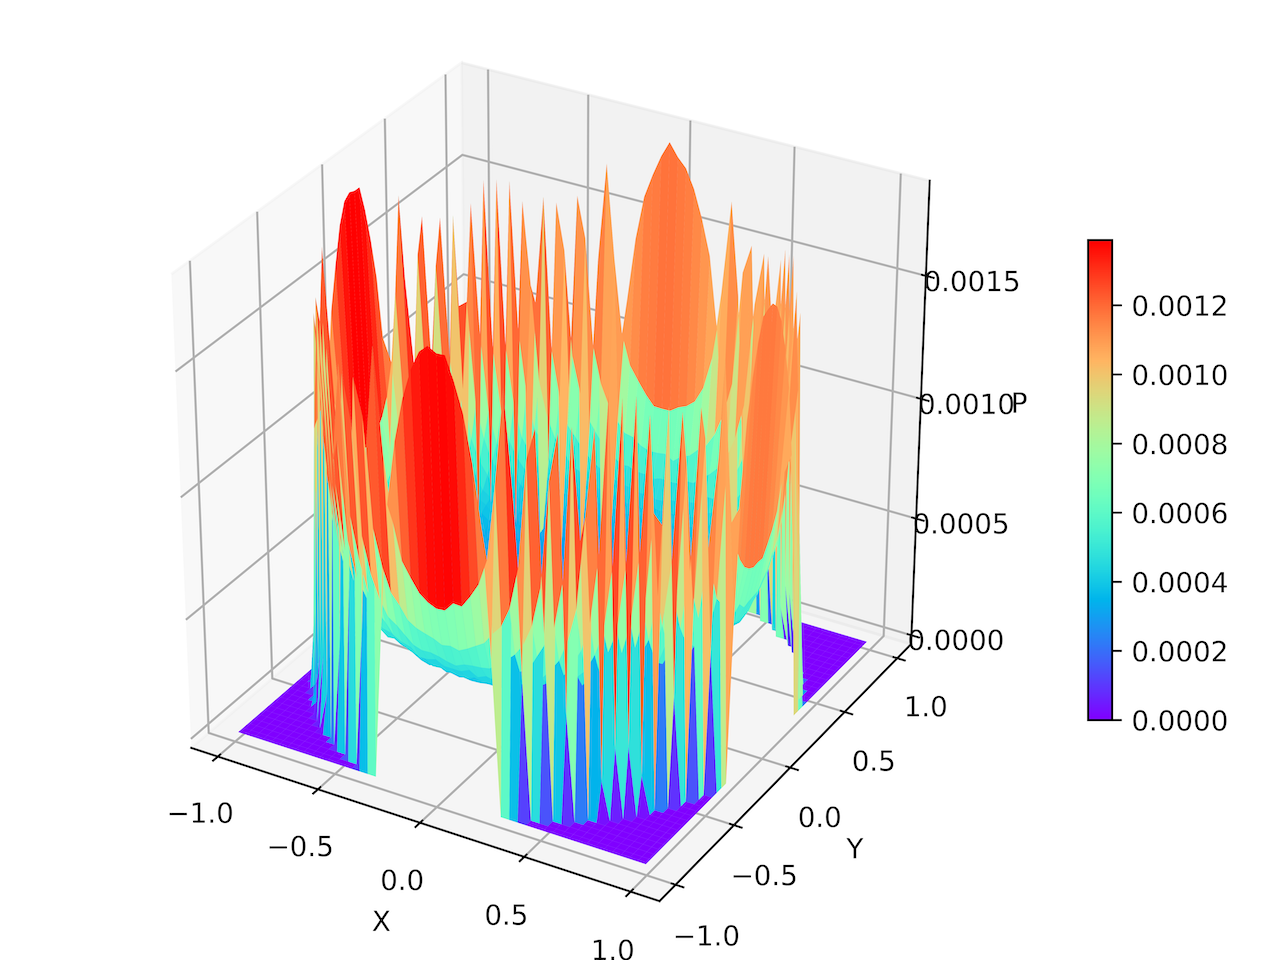
\includegraphics[width=5cm] {p107.png}
}
\subfigure[z方向视图]{
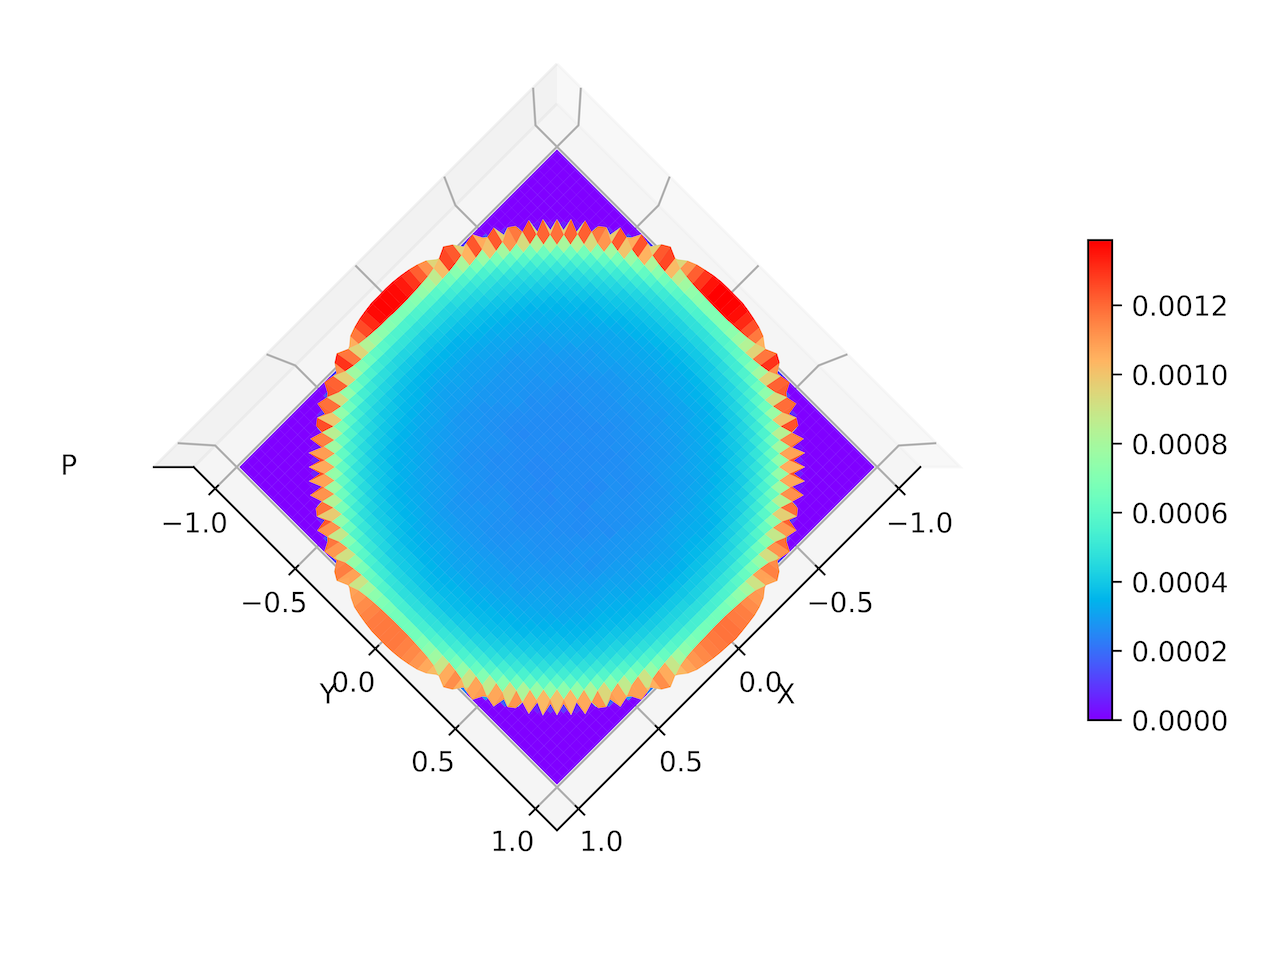
\includegraphics[width=5cm] {p107-v.png}
}      
\caption{16807 号产生器产生的球面上均匀分布的$10^{7}$随机点在$(x,y)$平面上的投影概率统计}      
\end{figure}

\begin{figure}[!htbp]   
\centering     
\subfigure[默认视图]{
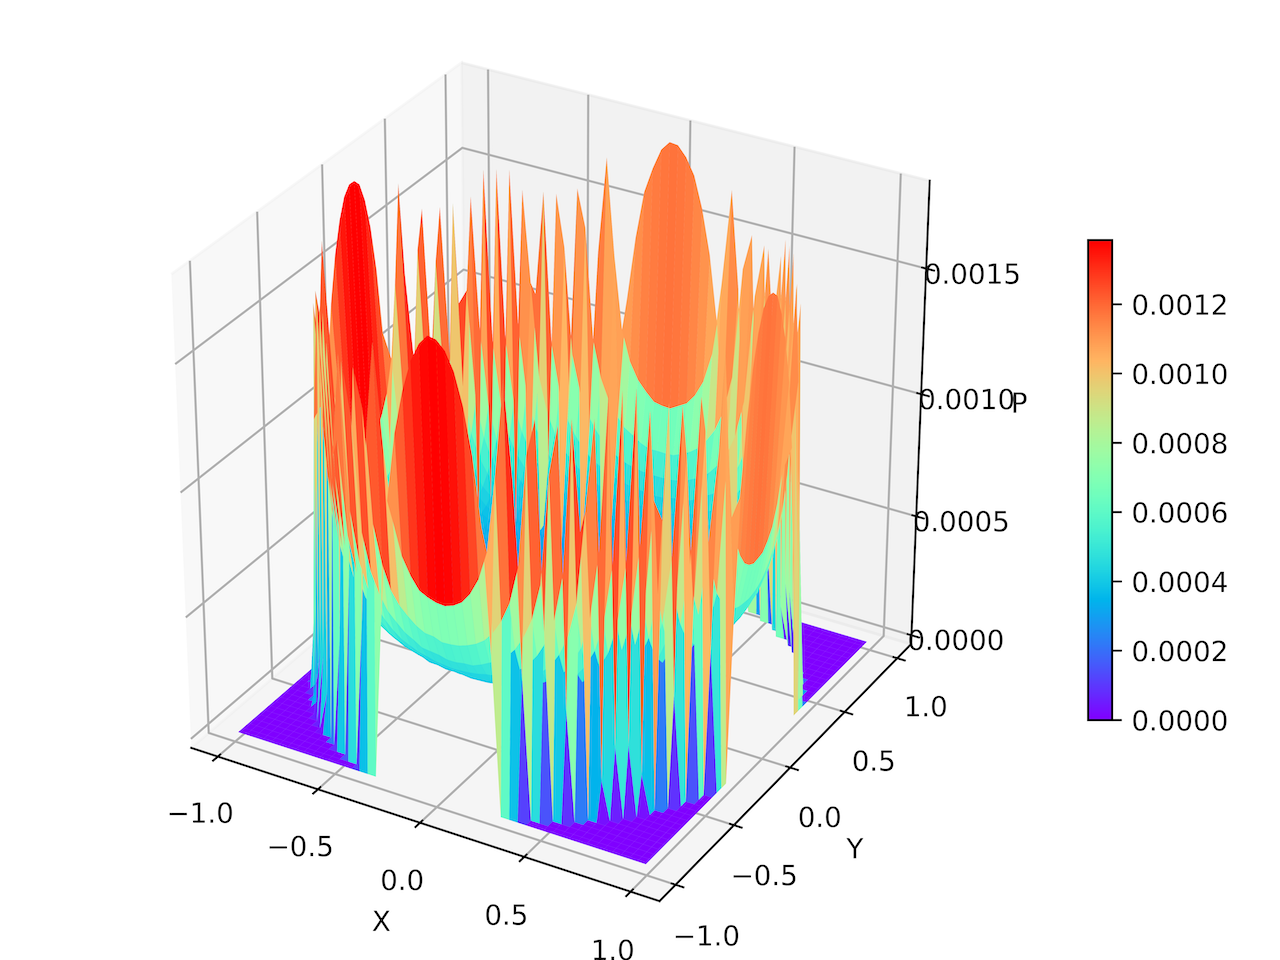
\includegraphics[width=5cm] {p108.png}
}
\subfigure[z方向视图]{
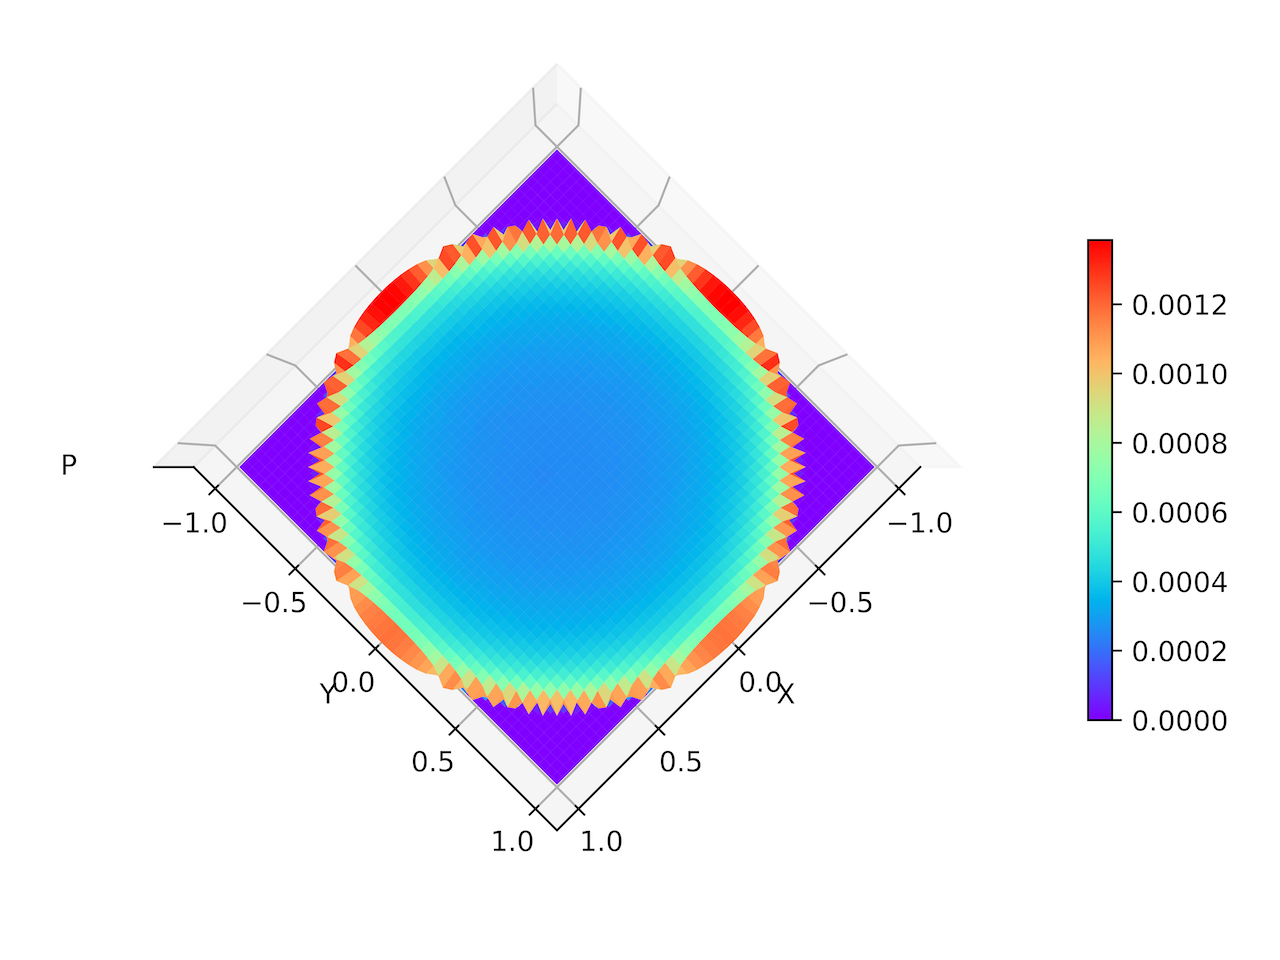
\includegraphics[width=5cm] {p108-v.png}
}      
\caption{16807 号产生器产生的球面上均匀分布的$10^{8}$随机点在$(x,y)$平面上的投影概率统计}      
\end{figure}

\newpage 对于$N=10^{8}$的情况,我们还做了其在$(x,y)$平面上的投影概率统计与理论概率统计的差值的图像:

\begin{figure}[!htbp]
\centering
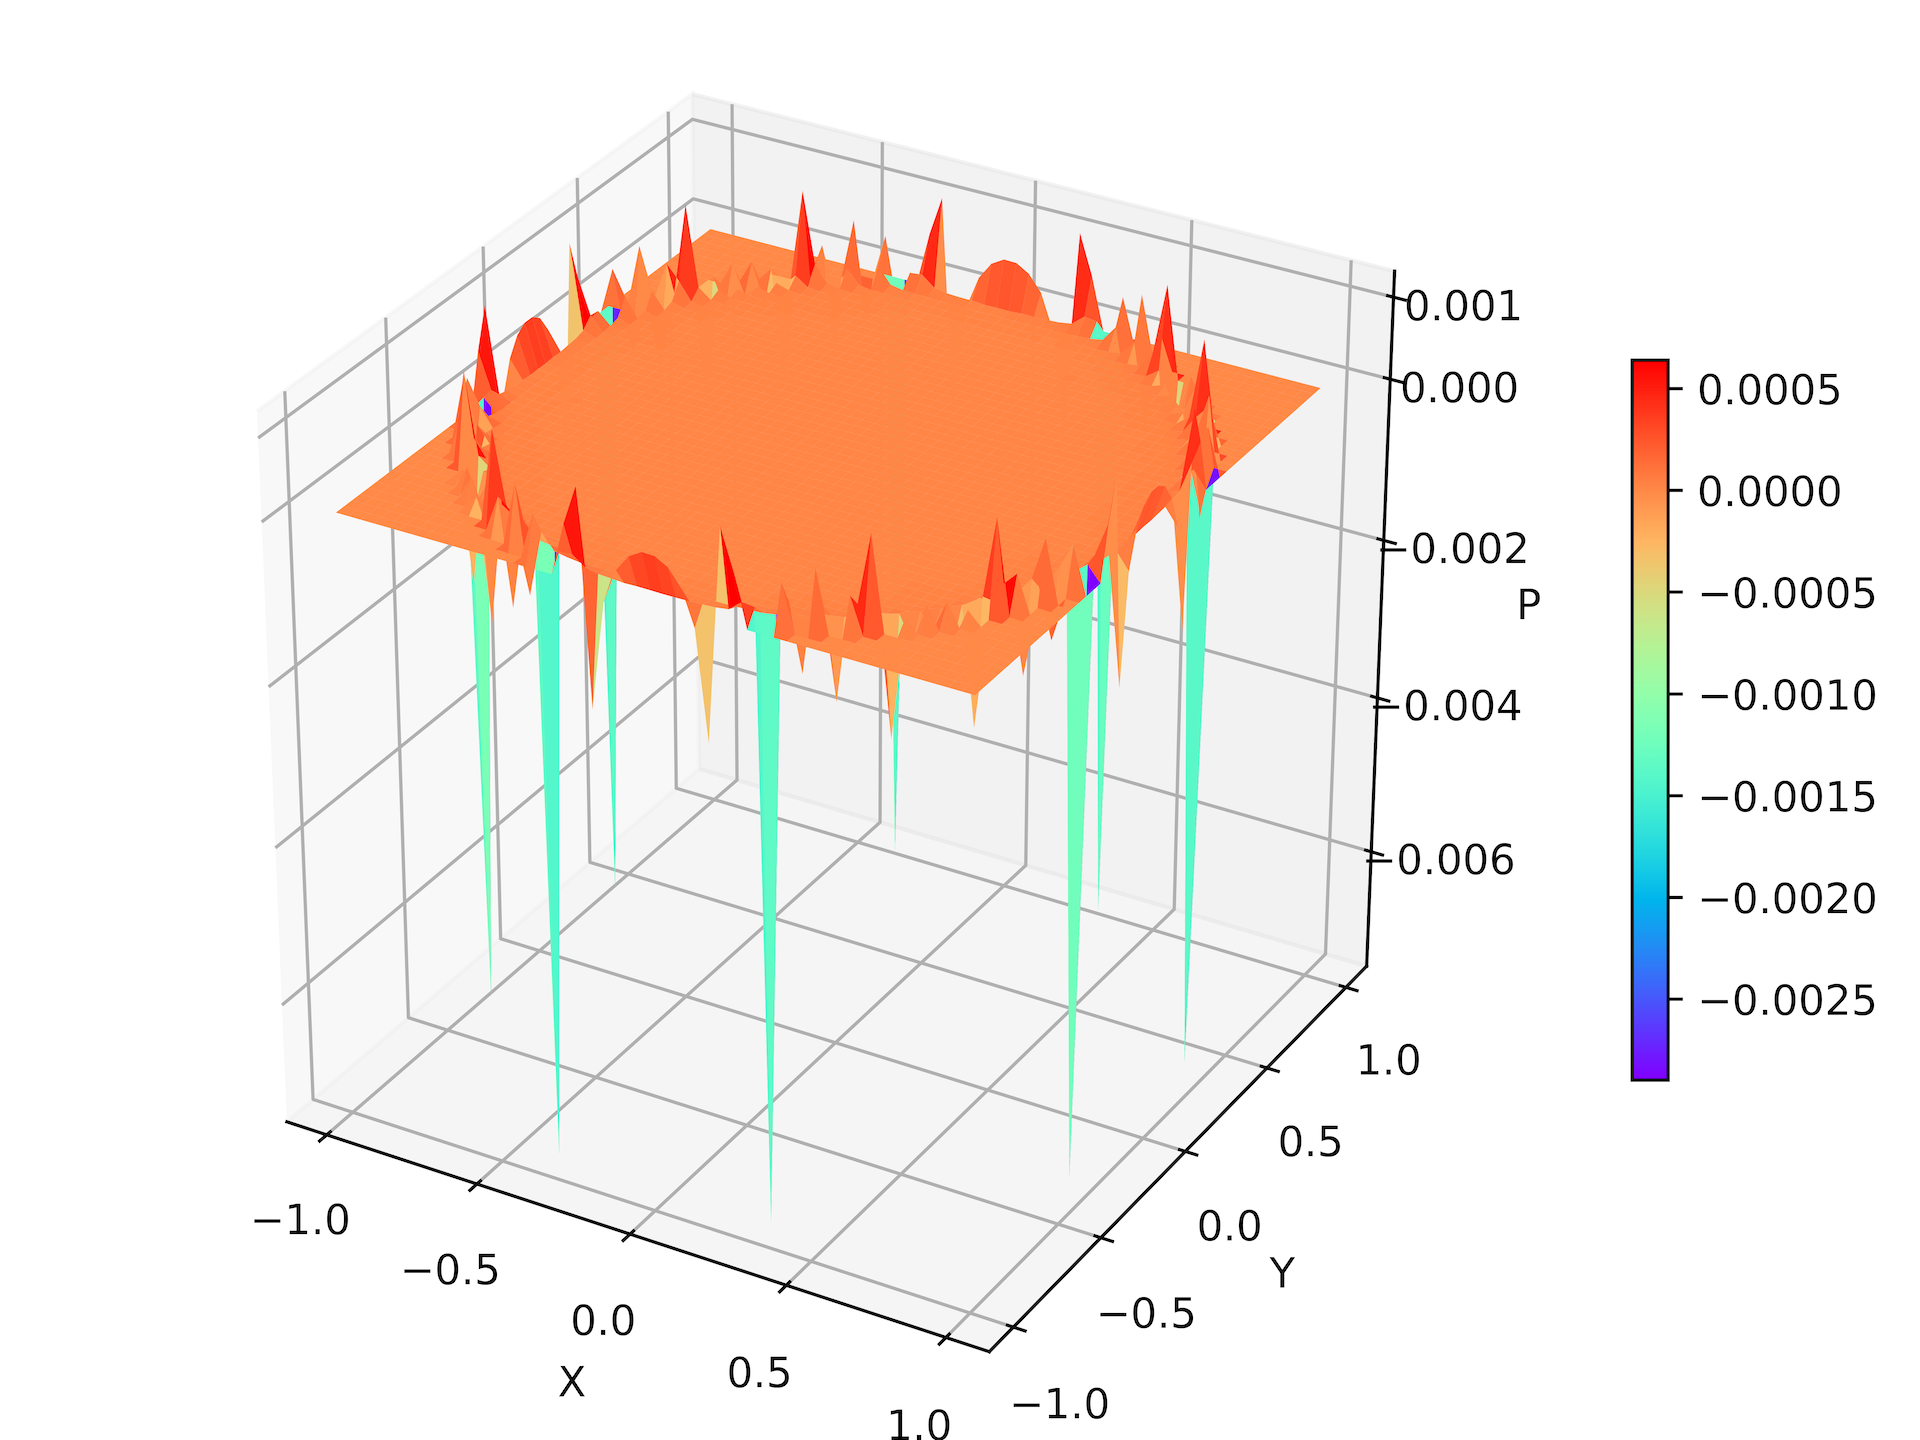
\includegraphics[width=7cm]{difference-8}
\caption{$N=10^{8}$时其$(x,y)$平面上的投影概率统计与理论概率统计的差值}	
\end{figure}

\newpage 其中理论概率统计由概率密度函数在剖分小区域中心的值并归一化得到,其为近似值。可看出两者的差除了在边缘附件比较大之外,其他地方差值基本为0.由于此概率密度分布在边缘处发散,故很难用数值的方法得到与理论值相差很小的结果,故此结果已经能够在一定程度上说明抽样得到的概率密度与理论密度一致。

 通过上节的理论推导与本节产生的图片,都能说明Marsaglia抽样方法产生的为球面上均匀分布的随机点。


\section{心得与体会}
通过此次作业结果,验证了Marsaglia 抽样方法确实能抽取球面上均匀分布的点。

通过编程作业,也更加熟悉了一些C语言和\LaTeX 。

\newpage
\section{附录}

\begin{appendices}



\section{产生随机数种子的C语言程序}
\begin{lstlisting}[language = C]
#include <stdio.h>
#include <stdlib.h>

//利用/dev/random 产生随机种子

int my_randomseed(int seed[],int n){

//seed为存储随机种子的数据,n为所需要种子的个数

		FILE * fp1 = fopen("/dev/random","r");

		for(int i=0;i<n;i++){
				fread(&seed[i], 1, sizeof(int), fp1);
		}

fclose(fp1);

return 0;
}

int main(){
int ranI[97];

my_randomseed(ranI,97);

FILE * fp;

fp = fopen("ranI.txt","w+");

for(int i=0;i<96;i++){
		fprintf(fp,"%d,",ranI[i]);
}

fprintf(fp,"%d",ranI[96]); //最后一个数据后不加 ","

fclose(fp);

return 0;

}	
\end{lstlisting}


\section{由上述程序产生的随机数文件1}
\label{971}
809576131,-1025892587,558213681,2056216731,-1652403892,-849346475,\\
-947398527,-2082766203,131013461,753913035,-634671236,995067675,-1025241712,\\
-57745909,187349022,-1487194468,174292363,-1523076266,-1381700026,1751317799,\\
812085654,-384904015,935241924,-2120102602,-1176252493,2084189454,-1308162651,\\
-721701972,1776417975,-1953284964,-1385173859,-1156931024,-272454405,-1527712783,\\
1040918716,966408491,-899150905,-1102248190,363327930,1940215723,924796768,861925965,\\
1030548881,1694050903,-1841641721,-5770120,448493076,1650846131,1012895949,\\
-2135767741,1924774890,-885687700,-219340479,-1417922044,-1101149761,1198019956,\\
-1522975896,842839847,2023490906,-1533950707,1267038558,1823349522,-1476843016,\\
786347740,1101867560,110498268,-1018391091,-1677263454,2117579346,-306068839,\\
569112568,-1031628950,1399939025,1102660725,-526224915,212410442,-968658785,\\
1808251768,166339465,-347114238,-1130541052,450232354,-684115741,-1313290066,\\
140916175,-1221648810,-1079940150,2079743593,414264974,-1639098679,142289346,\\
-2080694919,-345845707,-1201999899,1632261567,98605000,-1843368371


\section{由上述程序产生的随机数文件2}
\label{972}
-753424879,1872953453,608893860,597180613,2049110889,2140413464,1070133919,\\
-256067828,-1191457009,-574707053,-1410977199,1133706033,-404358309,1141209606,\\
-1604908044,2123698944,1542004389,894557832,-1972430293,-1544149044,-155439154,\\
2108522693,1220970092,697871479,-1502727159,1427890000,-1629207648,-132267497,\\
-749675637,1645721388,-1858854966,-2111533027,-151887203,-1412609570,-876296650,\\
-1227304997,701135804,1224292810,1805574955,-955336658,619132236,1948713847,\\
1737807285,845890383,-1491155579,-650075247,-1329866879,1910267507,-1879619968,\\
289013714,-24743716,1328343531,656220109,2045662973,-137884045,-1218521402,\\
1439903068,1203175289,-2098367843,1830857371,106846260,-1413985256,584445562,\\
-1141203261,-1584804986,-2109822000,-1573941759,1728136137,-54161293,-1017405251,\\
1652078157,1750018552,1594371093,1725375480,1445249495,-1114348371,-237895730,\\
1481242551,-1581295506,-970746651,397491742,462545489,-436989135,-1245824880,\\
-945627835,773430348,429365809,-108076855,620101426,1362478058,-923198353,\\
-1447637852,-1914066341,-1674823883,824439501,-461869274,-634359412
\section{C语言程序源码}

\begin{lstlisting}[language = C]
#include <stdio.h>
#include <stdlib.h>
#include <time.h>
#include <math.h>
#define a 16807
#define b 0
#define m 2147483647
#define r (m%a)
#define q (m/a)
#define Pi 3.1415926



int my_filereader_int(char str[],int num[],int n){
    FILE * fp;
    fp = fopen(str,"r");
    
    for(int i=0;i<n-1;i++)
    {
        fscanf(fp,"%d,",&num[i]);
        
    }
    fscanf(fp,"%d",&num[n-1]);    //最后一个数据后不加 ","
    fclose(fp);
    return 0;
}

int my_filewriter(char str[],double num[],int n){
    FILE * fp;
    fp = fopen(str,"w+");
    
    for(int i=0;i<n;i++)
    {
        if (i == (n-1)){
            fprintf(fp,"%lf",num[i]);
            break;
        }
        fprintf(fp,"%lf,",num[i]);
        
    }
    fclose(fp);
    return 0;
}




int  my_marsaglia_16807_sphere(int seed[],double ranu[],double ranv[],int n){
    for (int j = 0; j <= n; ) {
        if(seed[0] == m-1){
            if(a >=  b){    //由于Schrage方法只对z in (0,m-1)成立,故这里要讨论z == m-1的情况
                seed[0] = m + (b-a) % m;
            }
            else   seed[0] =  (b-a) % m;
            
        }
        if(seed[1] == m-1){
            if(a >=  b){    //由于Schrage方法只对z in (0,m-1)成立,故这里要讨论z == m-1的情况
                seed[1] = m + (b-a) % m;
            }
            else   seed[1] =  (b-a) % m;
            
        }
        seed[0] = ((a * (seed[0] % q) - r * (seed[0] /  q)) + b % m ) % m;
        seed[1] = ((a * (seed[1] % q) - r * (seed[1] /  q)) + b % m ) % m;
        if (seed[0] >= 0) {
            ranu[j] =  2*(seed[0] / (double)m) -1;
        }
        else{
            ranu[j] = 2*((seed[0] + m) / (double)m)-1 ;
        }
        
        if (seed[1] >= 0) {
            ranv[j] =  2*(seed[1] / (double)m)-1;
        }
        else{
            ranv[j] =  2*((seed[1] + m) / (double)m)-1;
        }
        if( pow(ranu[j],2) + pow(ranv[j],2) < 1 ) j++; //第j+1个元素满足舍选法条件后可继续向后写入数据,否则下一循环重新覆盖此数据
    }
    return 0;
}




//Fibonacci延迟器
int my_fibonacci_sphere(double ranu[],double ranv[],int ranI1[],int ranI2[],int n,int o,int p){
    int temp1;
    int temp2;
    int j = 0;
    for (int i = p; j < n; i++) {   //ranI[i % p]存放的为第i项
        
        temp1 = ranI1[i % p] - ranI1[(i % p+(p-o)) % p];  //递推式
        temp2 = ranI2[i % p] - ranI2[(i % p+(p-o)) % p];  //递推式
        
        if(temp1 >= 0) ranI1[i % p] = temp1 ;
        else ranI1[i % p] = temp1 + 1;  //递推得到的新结果放入ranI中i%p一项
        
        if(temp2 >= 0) ranI2[i % p] = temp2 ;
        else ranI2[i % p] = temp2 + 1;  //递推得到的新结果放入ranI中i%p一项
        
        if (ranI1[i % p] >= 0) {   //计算ran
            ranu[j] = 2*(ranI1[i % p] / (double) m)-1;
        } else {
            ranu[j] = 2*((ranI1[i % p] + m) / (double) m)-1;
        }
        
        if (ranI2[i % p] >= 0) {   //计算ran
            ranv[j] = 2*(ranI2[i % p] / (double) m)-1;
        } else {
            ranv[j] = 2*((ranI2[i % p] + m) / (double) m)-1;
        }
        
        if ( pow(ranu[j],2) + pow(ranv[j],2) < 1 ){
            j++;
        }
        
    }
    return 0;
}



int my_count(double ranx[],double rany[],double nk[][51],int n,int k){
    int x;
    int y;
    
for(int j=0;j<=k;j++){
    for(int e=0;e<=k;e++){
        nk[j][e] = 0;    //初始化数组
    }

}
for(int i=0;i<n;i++) {//计算各个实际频数
    x = floor((ranx[i]+1)/2*k);
    y = floor((rany[i]+1)/2*k);
    nk[x][y] += (double)1/n;
}
    return 0;
}




int main() {
    int N;  //产生总点数
    char str[50];
    printf("请输入您所需要的总点数:");
    while (!scanf("%d",&N)){   //简单的输入检查
        gets(str);
        printf("\nInput error,please try again\n");
        printf("请输入您所需要的总点数:");
    }
    
    int o,p;
inputpq:printf("请输入Marsaglia方法的延迟整数对[p,q](建议输入97,33)(英文逗号隔开):");
    while (!scanf("%d,%d",&o,&p)) {   //相对简单的输入检查
        gets(str);
        printf("\nInput error,please try again\n");
        printf("请输入Marsaglia方法的延迟整数对[p,q](建议值97,33)(英文逗号隔开):");
    }
    
    
    int temp;
    if(o > p){    //使 p > o
        temp = o;
        o = p;
        p=temp;
    }
    if( N-p < 3 ) {    //排除N相对于p,q太小的情况发生
        printf("输入的p,q值相对于总点数太大了,请重试!\n");
        goto inputpq;
    }

    
    if(N > 100000) printf("您输入的参数已接受,正在计算请稍后~\n");
    
    int seed[2] = {34028207,1677078722};
    
    double * ranu = malloc(sizeof(double)*(N+1));
    double * ranv = malloc(sizeof(double)*(N+1));
    double * ranx = malloc(sizeof(double)*N);
    double * rany = malloc(sizeof(double)*N);
    double * ranz = malloc(sizeof(double)*N);
    
    my_marsaglia_16807_sphere(seed, ranu, ranv, N);
    
    for (int i = 0;i<N;i++){  //计算x,y,z坐标值
        ranx[i] = 2*ranu[i]*pow(1-pow(ranu[i],2)-pow(ranv[i],2),0.5);
        rany[i] = 2*ranv[i]*pow(1-pow(ranu[i],2)-pow(ranv[i],2),0.5);
        ranz[i] = 1 - 2*( pow(ranu[i],2) + pow(ranv[i],2) );
    }
    
    double nk[51][51];
    my_count(ranx,rany,nk,N,50);  //统计在(x,y)平面上的y投影的分布,将[-1,1]*[-1,1]区间剖分为50*50个小区间统计
    
    FILE * fp;
    fp = fopen("hist.txt","w+");  //存放在(x,y)平面上的投影的分布
    
    for(int i=0;i<50;i++){   //统计16807方法产生的点在(x,y)平面上的投影的分布
        for(int j=0;j<50;j++){
            if( i==49 && j==49 ){
                fprintf(fp,"%lf",nk[j][i]);
                break;
            }
            fprintf(fp,"%lf ",nk[j][i]);
        }
        fprintf(fp,"\n");
    }
    fclose(fp);
    
    
    my_filewriter("ranx_16807.dat", ranx, N);
    my_filewriter("rany_16807.dat", rany, N);
    my_filewriter("ranz_16807.dat", ranz, N);
    /*    还可利用fibonacci产生器产生随机数方法抽样,此处略去
    int *ranI1 = malloc(sizeof(int) * p);      //用来存放递推数列
    int *ranI2 = malloc(sizeof(int) * p);
    my_filereader_int("ranI-1.txt",ranI1,p);   //读取之前利用"/dev/random"产生的初始随机数组
    my_filereader_int("ranI-2.txt",ranI2,p);
   
    my_fibonacci_sphere(ranu,ranv,ranI1,ranI2,N+1,o,p);
    for (int i = 0;i<N;i++){
        ranx[i] = 2*ranu[i]*pow(1-pow(ranu[i],2)-pow(ranv[i],2),0.5);
        rany[i] = 2*ranv[i]*pow(1-pow(ranu[i],2)-pow(ranv[i],2),0.5);
        ranz[i] = 1 - 2*( pow(ranu[i],2) + pow(ranv[i],2) );
    }

    my_filewriter("ranx_fibo.dat", ranx, N);
    my_filewriter("rany_fibo.dat", rany, N);
    my_filewriter("ranz_fibo.dat", ranz, N);
   */
    return 0;
}
\end{lstlisting}


\section{计算理论概率分布的C程序源码}

\begin{lstlisting}[language = C]
#include <stdio.h>
#include <math.h>
#define PI 3.1415926535


int my_filewriter_double(char str[],double num[],int n){
    FILE * fp;
    fp = fopen(str,"w+");
    
    for(int i=0;i<n;i++)
    {
        if (i == (n-1)){
            fprintf(fp,"%lf",num[i]);
            break;
        }
        fprintf(fp,"%lf ",num[i]);
        
    }
    fclose(fp);
    return 0;
}



int main(){
    int i = 0;
    double sum = 0;
    double ran[2500];
    int flag = 0;
    for (double y=-0.98;y<1;y += 0.04){
        for(double x = -0.98;x <1;x += 0.04){
            flag ++;
            if(x*x+y*y >=1){
                ran[i] = 0;
            }
            else{
                ran[i] = 1/(4*PI*sqrt(1-x*x-y*y));
                sum += 1/(4*PI*sqrt(1-x*x-y*y));
            }
            i++;
            
        }
    }
    printf("sum = %lf   flag = %d\n",sum,flag);
    for(int i =0;i<2500;i++){
        ran[i] = ran[i]/sum;
    }
    my_filewriter_double("op.txt", ran, 2500);
    return 0;
}
\end{lstlisting}


\section{可视化绘图python程序源码}

\begin{lstlisting}[language = python]

import matplotlib.pyplot as plt
from mpl_toolkits.mplot3d import Axes3D
import numpy as np
from IPython.core.pylabtools import figsize # import figsize
figsize(7, 7) # 设置 figsize
plt.rcParams['savefig.dpi'] = 1000 #图片像素
plt.rcParams['figure.dpi'] = 1000 #分辨率
# 默认的像素:[6.0,4.0],分辨率为100,图片尺寸为 600&400

fig = plt.figure()
ax = Axes3D(fig)
X = []
Y = []
Z = []

with open('problem 5/ranx_fibo.dat', 'r') as f:
    while True:
        lines = f.readline() # 整行读取数据
        if not lines:
            break
            pass
        tmp = [float(i) for i in lines.split(',')] # 将整行数据分割处理。
        X.append(tmp)  # 添加新读取的数据
        pass
    X = np.array(X) # 将数据从list类型转换为array类型。
pass

    
with open('problem 5/rany_fibo.dat', 'r') as f:
    while True:
        lines = f.readline() # 整行读取数据
        if not lines:
            break
            pass
        tmp = [float(i) for i in lines.split(',')] # 将整行数据分割处理。
        Y.append(tmp)  # 添加新读取的数据
        pass
    Y = np.array(Y) # 将数据从list类型转换为array类型。
pass

with open('problem 5/ranz_fibo.dat', 'r') as f:
    while True:
        lines = f.readline() # 整行读取数据
        if not lines:
            break
            pass
        tmp = [float(i) for i in lines.split(',')] # 将整行数据分割处理。
        Z.append(tmp)  # 添加新读取的数据
        pass
    Z = np.array(Z) # 将数据从list类型转换为array类型。
pass
    
       


# 绘制散点图
ax.scatter(X, Y, Z,s=0.0001)    #画散点图
ax.view_init(elev=90,azim=45)
ax.set_aspect('equal')   #设置三个坐标轴比例尺相同
ax.set_xlabel('X')
ax.set_ylabel('Y')
ax.set_zlabel('Z')
plt.savefig("1.png")

Z = []
with open('problem 5/hist.txt', 'r') as f:
    while True:
        lines = f.readline() # 整行读取数据
        if not lines:
            break
        temp = [float(i) for i in lines.split()] # 将整行数据分割处理,如果分割符是空格,括号里就不用传入参数,如果是逗号, 则传入‘,'字符。
        Z.append(temp)
    Z = np.array(Z) # 将数据从list类型转换为array类型。
pass


Z = Z.reshape(50,50)


X = np.linspace(-0.99, 0.99, 50)
Y = np.linspace(-0.99, 0.99, 50)
x, y = np.meshgrid(X, Y)
surf = ax.plot_surface(x, y, Z, rstride=1, cstride=1, cmap='rainbow')

ax.set_aspect('equal')   #设置三个坐标轴比例尺相同
ax.set_xlabel('X')
ax.set_ylabel('Y')
ax.set_zlabel('P')
ax.set_zticks([0, 0.0005, 0.001, 0.0015])
#ax.set_zticks([])
ax.set_yticks([-1, -0.5, 0, 0.5, 1])
ax.set_xticks([-1, -0.5, 0, 0.5, 1])
plt.colorbar(surf, shrink = 0.5)
#ax.view_init(elev=90,azim=45)
plt.savefig("p.png")	


\end{lstlisting}


\end{appendices}




\end{document}
